% !TEX root = My_thesis.tex

\input{template_settings/ch_preamble} % лучше не редактировать / please, keep unmodified

\setcounter{docType}{1} % лучше не редактировать / please, keep unmodified

%%%% Настройки автора / Author settings
%% 
\input{my_folder/my_settings} % добавляем свои команды / update your commands

\begin{document} % начало документа
	%%% Внесите свои данные - Input your data
%%
%%
\newcommand{\Author}{А.Б.\,Авдеева} % И.О. Фамилия автора 
\newcommand{\AuthorFull}{Авдеева Анастасия Борисовна} % Фамилия Имя Отчество автора
\newcommand{\AuthorFullDat}{Авдеевой Анастасии Борисовне} % Фамилия Имя Отчество автора в дательном падеже (Кому? Студенту...)
\newcommand{\AuthorFullVin}{Авдееву Анастасию Борисовну} % в винительном падеже (Кого? что?  Програмиста ...)
\newcommand{\AuthorPhone}{+7-953-374-63-72} % номер телефорна автора для оперативной связи  
\newcommand{\Supervisor}{И.О.\,Фамилия} % И. О. Фамилия научного руководителя
\newcommand{\SupervisorFull}{Фамилия Имя Отчество} % Фамилия Имя Отчество научного руководителя
\newcommand{\SupervisorVin}{И.О.\,Фамилию} % И. О. Фамилия научного руководителя  в винительном падеже (Кого? что? Руководителя ...)
\newcommand{\SupervisorJob}{должность} %
\newcommand{\SupervisorJobVin}{должность} % в винительном падеже (Кого? что?  Програмиста ...)
\newcommand{\SupervisorDegree}{степень} %
\newcommand{\SupervisorTitle}{звание} % 
%%
%%
%Руководитель, УТВЕРЖДАЮЩИЙ задание
\newcommand{\Head}{И.О.\,Фамилия} % И. О. Фамилия руководителя подразделения (руководителя ОП)
\newcommand{\HeadDegree}{Руководитель ОП}% Только должность:   
%Руководитель ОП % <- ПРАВИЛЬНЫЙ ВАРИАНТ ДЛЯ 09.03.03 и 09.04.03
%Заведующий % кафедрой
%Директор % Высшей школы
%Зам. директора
\newcommand{\HeadDep}{} % заменить на краткую аббревиатуру подразделения или ОСТАВИТЬ ПУСТЫМ, если утверждает руководитель ОП

%%% Руководитель, принимающий заявление
\newcommand{\HeadAp}{И.О.\,Фамилия} % И. О. Фамилия руководителя подразделения (руководителя ОП)
\newcommand{\HeadApDegree}{Руководитель ОП}% Только должность:   
%Руководитель ОП 
%Заведующий кафедрой
%Директор Высшей школы
\newcommand{\HeadApDep}{} % заменить на краткую аббревиатуру подразделения или оставить пустым, если утверждает руководитель ОП
%%% Консультант по нормоконтролю
\newcommand{\ConsultantNorm}{И.О.\,Фамилия} % И. О. Фамилия консультанта по нормоконтролю. ТОЛЬКО из числа ППС!
\newcommand{\ConsultantNormDegree}{должность, степень} %   
%%% Первый консультант
\newcommand{\ConsultantExtraFull}{Фамилия Имя Отчетство} % Фамилия Имя Отчетство дополнительного консультанта 
\newcommand{\ConsultantExtra}{И.О.\,Фамилия} % И. О. Фамилия дополнительного консультанта 
\newcommand{\ConsultantExtraDegree}{должность, степень} % 
\newcommand{\ConsultantExtraVin}{И.О.\,Фамилию} % И. О. Фамилия дополнительного консультанта в винительном падеже (Кого? что? Руководителя ...)
\newcommand{\ConsultantExtraDegreeVin}{должность, степень} %  в винительном падеже (Кого? что? Руководителя ...)
%%% Второй консультант
\newcommand{\ConsultantExtraTwoFull}{Фамилия Имя Отчетство} % Фамилия Имя Отчетство дополнительного консультанта 
\newcommand{\ConsultantExtraTwo}{И.О.\,Фамилия} % И. О. Фамилия дополнительного консультанта 
\newcommand{\ConsultantExtraTwoDegree}{должность, степень} % 
\newcommand{\ConsultantExtraTwoVin}{И.О.\,Фамилию} % И. О. Фамилия дополнительного консультанта в винительном падеже (Кого? что? Руководителя ...)
\newcommand{\ConsultantExtraTwoDegreeVin}{должность, степень} %  в винительном падеже (Кого? что? Руководителя ...)
\newcommand{\Reviewer}{И.О.\,Фамилия} % И. О. Фамилия резензента. Обязателен только для магистров.
\newcommand{\ReviewerDegree}{должность, степень} % 
%%
%%
\renewcommand{\thesisTitle}{Практическая работа}
\newcommand{\thesisDegree}{работа бакалавра}% магистерская диссертация %c 2020, И ТОЛЬКО для специалитата дипломный проект и дипломная работа
\newcommand{\thesisTitleEn}{Title of the thesis} %2020
\newcommand{\thesisDeadline}{18.12.2025} %Последний день преддипломной практики согласно учебному плану.
\newcommand{\thesisStartDate}{дд.мм.202X}
\newcommand{\thesisYear}{202X} % заменить на год защиты
\newcommand{\approveYear}{202\underline{\hspace*{0.01\textheight}}} % <- НЕ МЕНЯТЬ, ТОЛЬКО С 2030го :)
%%
%%
\newcommand{\group}{5130903/40003} % заменить вместо N номер группы
\newcommand{\thesisSpecialtyCode}{09.03.03}% код направления подготовки
\newcommand{\thesisSpecialtyTitle}{Прикладная информатика} % наименование направления/специальности
\newcommand{\thesisOPPostfix}{YY} % последние цифры кода образовательной программы (после <<_>>)
\newcommand{\thesisOPTitle}{Наименование направленности (профиля) образовательной программы}% наименование образовательной программы
%%
%%
\newcommand{\institute}{
Институт компьютерных наук и~кибербезопасности
%Гуманитарный институт
%Инженерно-строительный институт
%Институт биомедицинских систем и технологий
%Институт металлургии, машиностроения и транспорта
%Институт передовых производственных технологий
%Институт прикладной математики и механики
%Институт физики, нанотехнологий и телекоммуникаций
%Институт физической культуры, спорта и туризма
%Институт энергетики и транспортных систем
%Институт промышленного менеджмента, экономики и торговли
}%
%%
%%




%%% Задание ключевых слов и аннотации
%%
%%
%% Ключевых слов от 3 до 5 слов или словосочетаний в именительном падеже именительном падеже множественного числа (или в единственном числе, если нет другой формы) по правилам русского языка!!!
%%
%%
\newcommand{\keywordsRu}{статистический анализ, случайная выборка, C++, ООП, STL, численные методы} % ВВЕДИТЕ ключевые слова по-русски
%%
%%
\newcommand{\keywordsEn}{statistical analysis, random sampling, C++, OOP, STL, numerical methods} % ВВЕДИТЕ ключевые слова по-английски
%%
%%
%% Реферат ОТ 1000 ДО 1500 знаков на русский или английский текст
%%
%Реферат должен содержать:
%- предмет, тему, цель ВКР;
%- метод или методологию проведения ВКР:
%- результаты ВКР:
%- область применения результатов ВКР;
%- выводы.

\newcommand{\abstractRu}{В данной работе изложена сущность подхода к созданию консольного статистического калькулятора, предназначенного для формирования и анализа случайных выборок. Программная реализация основана на использовании языка C++ и принципов объектно-ориентированного программирования (ООП), что обеспечивает модульность и расширяемость функционала. Проведен анализ математических и численных методов для вычисления ключевых статистических характеристик. Изучена технология создания указанного класса программных систем. Разработана конкретная программная реализация, использующая Стандартную библиотеку шаблонов (STL), в частности контейнер std::vector для хранения данных.} % ВВЕДИТЕ текст аннотации по-русски
%%
%%
\newcommand{\abstractEn}{This work outlines the approach to creating a console-based statistical calculator designed for generating and analyzing random samples. The software implementation is based on the C++ language and the principles of Object-Oriented Programming (OOP), ensuring modularity and extensibility of the functionality. An analysis of mathematical and numerical methods for calculating key statistical characteristics has been conducted. The technology for creating this class of software systems was studied. A specific software implementation was developed, utilizing the Standard Template Library (STL), particularly the std::vector container for data storage.} % ВВЕДИТЕ текст аннотации по-английски


%%% РАЗДЕЛ ДЛЯ ОФОРМЛЕНИЯ ПРАКТИКИ
%Место прохождения практики
\newcommand{\PracticeType}{Отчет о прохождении % 
	%стационарной производственной (технологической (проектно-технологической)) %
	такой-то % тип и вид ЗАМЕНИТЬ
	практики}

\newcommand{\Workplace}{СПбПУ, ИКНК, ВШ ПИ} % TODO Rename this variable

% Даты начала/окончания
\newcommand{\PracticeStartDate}{%
дд.мм.гггг%
%	22.06.2020
}%
\newcommand{\PracticeEndDate}{%
	дд.мм.гггг%
%	18.07.2020%
}%
%%

\newcommand{\School}{
	Название высшей школы
%	Высшая школа программной инженерии 
}
\newcommand{\practiceTitle}{Тема практики}


%% ВНИМАНИЕ! Необходимо либо заменить текст аннотации (ключевых слов) на русском и английском, либо удалить там весь текст, иначе в свойства pdf-отчета по практике пойдет шаблонный текст.

%%% Не меняем дальнейшую часть - Do not modify the rest part
%%
%%
%%
%%
\ifnumequal{\value{docType}}{1}{% Если ВКР, то...
	\newcommand{\DocType}{Курсовая работа}
	\newcommand{\pdfDocType}{\DocType~(\thesisDegree)} %задаём метаданные pdf файла
	\newcommand{\pdfTitle}{\thesisTitle}
}{% Иначе 
	\newcommand{\DocType}{\PracticeType}
	\newcommand{\pdfDocType}{\DocType} %задаём метаданные pdf файла
	\newcommand{\pdfTitle}{\practiceTitle}
}%
\newcommand{\HeadTitle}{\HeadDegree~\HeadDep}
\newcommand{\HeadApTitle}{\HeadApDegree~\HeadApDep}
\newcommand{\thesisOPCode}{\thesisSpecialtyCode\_\thesisOPPostfix}% код образовательной программы
\newcommand{\thesisSpecialtyCodeAndTitle}{\thesisSpecialtyCode~\thesisSpecialtyTitle}% Код и наименование направления/специальности
\newcommand{\thesisOPCodeAndTitle}{\thesisOPCode} % код и наименование образовательной программы
%%
%%
\hypersetup{%часть болка hypesetup в style
		pdftitle={\pdfTitle},    % Заголовок pdf-файла
		pdfauthor={\AuthorFull},    % Автор
		pdfsubject={\pdfDocType. Шифр и наименование направления подготовки: \thesisSpecialtyCodeAndTitle. \abstractRu},      % Тема
		pdfcreator={LaTeX, SPbPU-student-thesis-template},     % Приложение-создатель
%		pdfproducer={},  % Производитель, Производитель PDF % будет выставлена автоматически
		pdfkeywords={\keywordsRu}
}
%%
%%
%% вспомогательные команды
\newcommand{\firef}[1]{рис.\ref{#1}} %figure reference
\newcommand{\taref}[1]{табл.\ref{#1}}	%table reference
%%
%%
%% Архивный вариант задания ключевых слов, аннотации и благодарностей 
% Too hard to export data from the environment to pdf-info
% https://tex.stackexchange.com/questions/184503/collecting-contents-of-environment-and-store-them-for-later-retrieval
%заменить NewEnviron на newenvironment для распознавания команды в TexStudio
%\NewEnviron{keywordsRu}{\noindent\MakeUppercase{\BODY}}
%\NewEnviron{keywordsEn}{\noindent\MakeUppercase{\BODY}}
%\newenvironment{abstractRu}{}{}
%\newenvironment{abstractEn}{}{}
%\newenvironment{acknowledgementsRu}{\par{\normalfont \acknowledgements.}}{}
%\newenvironment{acknowledgementsEn}{\par{\normalfont \acknowledgementsENG.}}{}


%%% Переопределение именований %%% Не меняем - Do not modify
%\newcommand{\Ministry}{Минобрнауки России} 
\newcommand{\Ministry}{Министерство науки и высшего образования Российской~Федерации} %с 2020
\newcommand{\SPbPU}{Санкт-Петербургский политехнический университет Петра~Великого}
\newcommand{\SPbPUOfficialPrefix}{Федеральное государственное автономное образовательное учреждение высшего образования}
\newcommand{\SPbPUOfficialShort}{ФГАОУ~ВО~<<СПбПУ>>}
%% Пробел между И. О. не допускается.
\renewcommand{\alsoname}{см. также}
\renewcommand{\seename}{см.}
\renewcommand{\headtoname}{вх.}
\renewcommand{\ccname}{исх.}
\renewcommand{\enclname}{вкл.}
\renewcommand{\pagename}{Pages}
\renewcommand{\partname}{Часть}
\renewcommand{\abstractname}{\textbf{Аннотация}}
\newcommand{\abstractnameENG}{\textbf{Annotation}}
\newcommand{\keywords}{\textbf{Ключевые слова}}
\newcommand{\keywordsENG}{\textbf{Keywords}}
\newcommand{\acknowledgements}{\textbf{Благодарности}}
\newcommand{\acknowledgementsENG}{\textbf{Acknowledgements}}
\renewcommand{\contentsname}{Content} % 
%\renewcommand{\contentsname}{Содержание} % (ГОСТ Р 7.0.11-2011, 4)
%\renewcommand{\contentsname}{Оглавление} % (ГОСТ Р 7.0.11-2011, 4)
\renewcommand{\figurename}{Рис.} % Стиль СПбПУ
%\renewcommand{\figurename}{Рисунок} % (ГОСТ Р 7.0.11-2011, 5.3.9)
\renewcommand{\tablename}{Таблица} % (ГОСТ Р 7.0.11-2011, 5.3.10)
%\renewcommand{\indexname}{Предметный указатель}
\renewcommand{\listfigurename}{Список рисунков}
\renewcommand{\listtablename}{Список таблиц}
\renewcommand{\refname}{\fullbibtitle}
\renewcommand{\bibname}{\fullbibtitle}

\newcommand{\chapterEnTitle}{Сhapter title} % <- input the English title here (only once!) 
\newcommand{\chapterRuTitle}{Название главы}          % <- введите 
\newcommand{\sectionEnTitle}{Section title} %<- input subparagraph title in english
\newcommand{\sectionRuTitle}{Название подраздела} % <- введите название подраздела по-русски
\newcommand{\subsectionEnTitle}{Subsection title} % - input subsection title in english
\newcommand{\subsectionRuTitle}{Название параграфа} % <- введите название параграфа по-русски
\newcommand{\subsubsectionEnTitle}{Subsubsection title} % <- input subparagraph title in english
\newcommand{\subsubsectionRuTitle}{Название подпараграфа} % <- введите название подпараграфа по-русски % Заполнить сведения, 


	%%% Титульник ВКР / Thesis title 
%%
%% добавить лист в pdf-навигацию 
%% add to pdf navigation menu
%%
\pdfbookmark[-1]{\pdfTitle}{tit}
%%
\thispagestyle{empty}%
\makeatletter
\newgeometry{top=2cm,bottom=2cm,left=3cm,right=1cm,headsep=0cm,footskip=0cm}
\savegeometry{NoFoot}%
\makeatother


% %%% Распечатать версию документа / Print document version
% %%
% \begin{flushright}
% %	\vspace{0pt plus0.1fill}
% 	\boxed{\small
% 		\begin{tabular}{r} 
% 			\textbf{Пример ВКР <<SPbPU-student-thesis-template>>.} %\\ % перенос на новую строку
% 			\textbf{Версия от \today % \; время:  \currenttime. % время версии
% 			}
% 		\end{tabular}
% 	} %end boxed
% %	\vspace*{-5pt} % раскомментировать, если не хватает места
% 	\vspace{0pt plus0.1fill} % раскоментировать, если хватает места
% \end{flushright}

% {\centering%
% 	\Ministry\\
% 	\SPbPU\\
% 	{%\bfseries %2020 - указание на изменения, которые могут быть введены в 2020 году
% 		\institute}
% \par}%


% \vspace{0pt plus1fill} %число перед fill = кратность относительно некоторого расстояния fill, кусками которого заполнены пустые места


% \noindent
% \begin{minipage}{\linewidth}
% 	\vspace{\mfloatsep} % интервал 
% 	\begin{tabularx}{\linewidth}{Xl}
% 	&Работа допущена к защите     \\
% 	&\HeadTitle     \\			
% 	&\underline{\hspace*{0.1\textheight}} \Head     \\
% 	&<<\underline{\hspace*{0.05\textheight}}>> \underline{\hspace*{0.1\textheight}} \approveYear~г.  \\ 
% 	\end{tabularx}
% 	\vspace{\mfloatsep} % интервал 	
% \end{minipage}


% \vspace{0pt plus2fill} %


% {\centering%
	
% 	\MakeUppercase{\bfseries{}\DocType} \\ 
% 	\MakeUppercase{\normalfont{}\thesisDegree}%


% %\intervalS% %ОБЯЗАТЕЛЬНО ДОБАВИТЬ ОТСТУП, ЕСЛИ ХВАТАЕТ МЕСТА
% {\centering%
% 	\MakeUppercase{\bfseries{\thesisTitle}}}%

% }\par%

% %\intervalS% %ОБЯЗАТЕЛЬНО ДОБАВИТЬ ОТСТУП, ЕСЛИ ХВАТАЕТ МЕСТА
% %по специальности % для специалистов
% \noindent	по направлению подготовки 09.03.03 Прикладная информатика\\% для бакалавров и магистров 
% %\noindent Направленность  % для специалистов
% \noindent	Направленность (профиль)	\thesisOPCodeAndTitle % для бакалавров и магистров
% % Лучше по~профилю, но что делать, так составили Положение
% \par%





% \vspace{4mm plus2fill}%

% \noindent
% \begin{tabularx}{\linewidth}{lXl}
% 	Выполнил              &	   &             \\
% 	студент гр. 5130903/40003    &    & А.Б. Авдеева     \\[\mfloatsep]

% 	Руководитель 		  &    &             \\
% 	\SupervisorJob,		  &    &             \\
% 	\SupervisorDegree, \SupervisorTitle\footnote{Должность указывают сокращенно, учёную степень и звание ---~при наличии, а~подразделения ---~аббревиатурами. <<СПбПУ>> и~аббревиатуры институтов не добавляют.} 	  &    & \Supervisor \\[\mfloatsep]
	
% 	Консультант\footnote{Оформляется по решению руководителя ОП или подразделения. Только 1 категория: <<Консультант>>. В исключительных случаях можно указать <<Научный консультант>> (должен иметь степень). Без печати и заверения подписи.}		  &    & 			 \\
% 	\ConsultantExtraDegree 	  &    & \ConsultantExtra\\[\mfloatsep]
	
% 	Консультант  &    &  \\   	
% 	по нормоконтролю\footnote{Обязателен, из числа ППС по решению руководителя ОП или подразделения. Должность и степень не указываются. Сведения помещаются в последнюю строчку по порядку. Рецензенты не указываются.}  		 	  &    & \ConsultantNorm  % обязателен
% \end{tabularx} %


% %
% \vspace{0pt plus4fill}% 


% \begin{center}%
% 	Санкт-Петербург \\
% 2025 \\
% \end{center}%
% \restoregeometry
% \newpage


% --- Верхняя часть ---
\vspace*{10mm}
\begin{center}
{\fontsize{14pt}{16pt}\selectfont
Санкт-Петербургский политехнический университет Петра\\
Великого\\[4mm]
Институт компьютерных наук и кибербезопасности\\
Высшая школа программной инженерии
}
\end{center}

% --- Заголовки по центру ---
\vspace*{10mm}
\begin{center}
{\bfseries\fontsize{16pt}{18pt}\selectfont Приоритизация тестовых случаев на основе генетического алгоритма}\\[3mm]
% {\bfseries\fontsize{14pt}{16pt}\selectfont Статический и динамический анализ приложения}\\[3mm]
{\fontsize{14pt}{16pt}\selectfont по дисциплине «Методы тестирования программного обеспечения»}
\end{center}

% --- НИЖНИЙ БЛОК КАК НА СКРИНЕ (компилируется нормально) ---
\vspace*{85mm}

\noindent
\begin{tabular*}{\textwidth}{@{}p{0.68\textwidth}@{\extracolsep{\fill}}>{\raggedleft\arraybackslash}p{0.30\textwidth}@{}}
\textbf{Выполнил} & \\[6pt]
студент гр.5130903/40003 & Я. М. Качанов\\[18pt]

\textbf{Руководитель} & \\[6pt]
старший преподаватель & \\[2pt]
ВШПИ & В. А. Пархоменко\\
\end{tabular*}

\vfill
\begin{center}
Санкт-Петербург – 2026
\end{center}
					 % Титульный лист


	% \input{my_folder/task}					 % Задание 


	% \input{my_folder/summary}			 	 % Реферат 


	\input{my_folder/contents}  	         % Оглавление


	\chapter*{Введение} % * не простaвляет номер
\addcontentsline{toc}{chapter}{Введение} % вносим в содержaние


\textbf{Актуальность}. Регрессионное тестирование является неотъемлемой частью процесса разработки 
программного обеспечения: после каждого изменения кода необходимо убедиться, что существующая 
функциональность не нарушена. По мере роста проекта тестовый набор увеличивается экспоненциально, 
что делает полный повторный прогон тестов дорогостоящим и времязатратным. Приоритизация тестовых случаев 
(Test Case Prioritization, TCP) позволяет упорядочить выполнение тестов таким образом, чтобы дефекты 
обнаруживались как можно раньше, не исключая ни одного теста из набора. Применение эволюционных методов 
оптимизации, в частности генетических алгоритмов, открывает возможность учитывать одновременно несколько 
критериев качества при формировании порядка выполнения тестов.

\textbf{Предмет исследования}. Методы приоритизации тестовых случаев на основе генетического алгоритма с 
многокомпонентной фитнесс-функцией, включающей покрытие кода, оценку вероятности дефектов (fault-proneness) 
и структурное разнообразие тестов (diversification) на основе расстояния Жаккара.

\textbf{Цель исследования}. Разработка и экспериментальная оценка алгоритма приоритизации тестовых случаев, 
превосходящего базовый генетический алгоритм и жадный алгоритм дополнительного покрытия по метрикам APFD и 
APFDc на реальных наборах данных.

\textbf{Зaдaчи:}
\begin{enumerate}[1.]
	\item Изучить существующие методы приоритизации тестовых случаев и метрики оценки их эффективности.
	\item Разработать фитнесс-функцию генетического алгоритма, учитывающую покрытие кода, fault-proneness и структурное разнообразие тестов.
	\item Реализовать алгоритм на языке Java с поддержкой загрузки данных в форматах CSV и JSON.
	\item Провести сравнительный эксперимент на разных наборах данных.
	\item Проанализировать результаты и определить условия применимости предложенного подхода.
\end{enumerate} 
	    	 % Введение

	%% Начало основной части
	\chapter{Анализ существующих методов} \label{ch1}

В данной главе рассматриваются основные подходы к приоритизации тестовых случаев, их преимущества и ограничения. 
В параграфе~\ref{ch1:sec1} описана задача регрессионного тестирования и приоритизации тестовых случаев.
В параграфе~\ref{ch1:sec2} рассмотрены существующие методы приоритизации и их ограничения.

\section{Регрессионное тестирование и приоритизация тестовых случаев} 
\label{ch1:sec1}

Регрессионное тестирование --- процесс повторного выполнения тестов после внесения изменений в программный код с 
целью подтверждения того, что ранее работавшая функциональность не нарушена. По мере развития проекта объём 
тестового набора растёт, что делает полный повторный прогон нецелесообразным с точки зрения временных и 
вычислительных затрат.

Для решения данной проблемы используются три основных подхода: минимизация тестового набора (Test Suite Minimization), 
отбор тестов (Test Case Selection) и приоритизация тестовых случаев (Test Case Prioritization, TCP). 
В отличие от первых двух, TCP не исключает тесты из набора, а только упорядочивает их выполнение по некоторому 
критерию, сохраняя полноту покрытия.

\section{Существующие методы приоритизации}\label{ch1:sec2}

Среди методов приоритизации выделяют несколько классов, каждый из которых имеет характерные ограничения.

Случайный поиск (Random Search) упорядочивает тесты в произвольном порядке без учёта каких-либо критериев. 
Несмотря на простоту, он служит нижней границей сравнения --- любой разумный алгоритм приоритизации должен 
превосходить случайный порядок.

Жадные алгоритмы на основе покрытия кода упорядочивают тесты по убыванию числа новых покрываемых элементов. 
Алгоритм дополнительного покрытия (Additional) на каждом шаге выбирает тест с максимальным числом ещё не покрытых
элементов --- это простой и эффективный подход, однако он не учитывает вероятность дефектов и принимает локально 
оптимальные решения, не гарантируя глобального оптимума.

Эволюционные методы, в частности генетические алгоритмы, рассматривают задачу TCP как задачу оптимизации перестановок.
В работе~\cite{paygude2020} рассматривается применение ГА к набору данных BigFaultMatrix, показано превосходство 
над случайным поиском и алгоритмами hill climbing. Вместе с тем фитнесс-функция учитывает только скорость 
обнаружения дефектов, не принимая во внимание вероятность дефектов и структурное разнообразие тестов.

В статье~\cite{mahdieh2021} рассматривается подход CovClustering, в котором вероятность дефектов (fault-proneness)
методов оценивается на основе анализа влияния изменений (Change Impact Analysis, CIA). Подход учитывает вероятность
дефектов, однако использует кластеризацию вместо эволюционного поиска, что ограничивает возможности глобальной 
оптимизации порядка тестов.

Таким образом, ни один из рассмотренных методов не сочетает одновременно эволюционный поиск, учёт вероятности 
дефектов и структурное разнообразие тестов. Устранение этих ограничений является целью настоящей работы.	         	 % Глава 1
	\ContinueChapterBegin % размещать главы <<подряд>> 
	\chapter{Постановка задачи} \label{ch2}

В данной главе приведена формальная постановка задачи приоритизации тестовых случаев и определены метрики
оценки эффективности. В параграфе~\ref{ch2:sec1} дано формальное определение задачи. В параграфе~\ref{ch2:sec2} 
описаны метрики APFD и APFDc.

\section{Формальное определение} \label{ch2:sec1}

Пусть $T = \{t_1, t_2, \ldots, t_n\}$ --- тестовый набор из $n$ тестовых случаев. 
Каждый тестовый случай $t_i$ характеризуется множеством покрываемых методов $M_i \subseteq M$, вероятностью 
дефектов $r_i \in [0, 1]$ и временем выполнения $c_i > 0$.

Задача приоритизации состоит в нахождении перестановки $T^*$: $$T^* = \arg\max_{T' \in \Pi(T)} f(T')$$
где $\Pi(T)$ --- множество всех перестановок $T$, целевая функция: 
$$f(T') = w_c \cdot \text{Cov}(T') + w_r \cdot \text{FP}(T') + w_d \cdot \text{Div}(T'), \quad w_c + w_r + w_d = 1$$

\section{Метрики оценки эффективности} \label{ch2:sec2}

Основной метрикой оценки является APFD (Average Percentage of Faults 
Detected)~\cite{elbaum2002}:
\begin{equation}\label{eq:apfd}
\text{APFD} = 1 - \frac{\sum_{i=1}^{m} TF_i}{n \cdot m} + \frac{1}{2n}
\end{equation}
где $n$ --- количество тестов, $m$ --- количество дефектов, $TF_i$ --- позиция теста, первым обнаружившего
$i$-й дефект. Значение APFD близкое к~1 означает, что дефекты обнаруживаются в начале выполнения набора.

Метрика APFDc расширяет APFD с учётом стоимости выполнения каждого теста:
$$\text{APFDc} = \frac{\sum_{i=1}^{m} \left( t_{TF_i} - \frac{c_{TF_i}}{2} \right)}{T_{total} \cdot m}$$
где $t_{TF_i}$ --- суммарное время выполнения тестов до момента обнаружения $i$-го дефекта, $c_{TF_i}$ --- 
время выполнения теста обнаружившего дефект, $T_{total}$ --- суммарное время выполнения всего набора.	         	 % Глава 2
	\chapter{Предлагаемый метод} \label{ch3}

В данной главе описан разработанный алгоритм приоритизации тестовых случаев GA-FP+Div, представляющий 
собой генетический алгоритм с улучшенной многокомпонентной фитнесс-функцией.

\section{Фитнесс-функция}\label{ch3:sec1}

Фитнесс-функция оценивает качество предложенной последовательности тестов по трём нормализованным компонентам. 
Использование нескольких компонент позволяет учитывать не только покрытие кода, но и рискованность покрываемых 
методов и структурное разнообразие тестов.

\textbf{Покрытие кода} ($\text{Cov}$) --- доля уникальных методов, покрытых последовательностью тестов, от 
общего числа методов проекта:
$$\text{Cov}(T') = \frac{|\bigcup_{i=1}^{n} M_i|}{|M|}$$

Числитель --- количество уникальных методов, покрытых хотя бы одним тестом из последовательности. 
Знаменатель --- общее число методов в проекте. Результат нормализован к диапазону $[0, 1]$.

\textbf{Вероятность дефектов} ($\text{FP}$) --- средняя вероятность дефектов первых $k$ тестов последовательности:
$$\text{FP}(T') = \frac{1}{k}\sum_{i=1}^{k} r_{\pi(i)}$$

где $r_{\pi(i)}$ --- вероятность дефектов $i$-го теста в последовательности, оцениваемая на основе анализа 
влияния изменений CIA (Change Impact Analysis). Компонента максимизирует вероятность того, что наиболее 
рискованные тесты выполняются первыми.

\textbf{Структурное разнообразие} ($\text{Div}$) --- среднее расстояние Жаккара между соседними тестами в 
первых $k$ позициях:
$$\text{Div}(T') = \frac{1}{k-1}\sum_{i=1}^{k-1} d_J(M_{\pi(i)}, M_{\pi(i+1)})$$

где расстояние Жаккара определяется как:
$$d_J(A, B) = 1 - \frac{|A \cap B|}{|A \cup B|}$$

Значение $d_J = 0$ означает что тесты покрывают одинаковые методы, $d_J = 1$ --- покрытия не пересекаются. 
Компонента стимулирует алгоритм чередовать тесты с различным покрытием, снижая дублирование в начале последовательности.

Все три компоненты нормализованы к диапазону $[0, 1]$. Итоговый фитнесс вычисляется как взвешенная сумма:
$$f(T') = w_c \cdot \text{Cov}(T') + w_r \cdot \text{FP}(T') + w_d \cdot \text{Div}(T')$$

где $w_c + w_r + w_d = 1$, $w_c, w_r, w_d \geq 0$. В настоящей 
работе приняты значения $w_c = 0{,}2$, $w_r = 0{,}6$, $w_d = 0{,}2$, 
$k = 10$.

\section{Операторы генетического алгоритма} \label{ch3:sec2}

Генетический алгоритм оперирует популяцией из $N$ особей, каждая из которых представляет собой перестановку 
тестового набора $T$. На каждом поколении популяция обновляется с помощью операторов селекции, кроссовера и мутации.

\textbf{Инициализация.} Начальная популяция из $N$ особей формируется случайным перемешиванием тестового набора $T$.
Использование фиксированного зерна генератора случайных чисел обеспечивает воспроизводимость результатов.

\textbf{Селекция.} Используется турнирная селекция с размером турнира $s = 3$: случайно выбираются $s$ особей, 
из которых в следующее поколение передаётся особь с наибольшим значением фитнесса. Турнирная селекция обеспечивает 
селективное давление без полного исключения слабых особей.

\textbf{Кроссовер.} Применяется оператор OX (Order Crossover), сохраняющий валидность перестановки. 
Алгоритм OX работает следующим 
образом:
\begin{enumerate}
    \item Случайно выбирается сегмент $[\alpha, \beta]$ из первого 
    родителя $P_1$ и копируется в потомка $C$ на те же позиции.
    \item Оставшиеся позиции $C$ заполняются элементами из второго 
    родителя $P_2$ в порядке их появления, пропуская элементы уже 
    присутствующие в сегменте.
\end{enumerate}

Например, для $P_1 = [t_3, t_1, t_5, t_2, t_4]$ и 
$P_2 = [t_2, t_4, t_1, t_5, t_3]$ при сегменте $[1, 3]$:
$$C = [t_2, \underbrace{t_1, t_5, t_2}_{\text{сегмент из } P_1}, t_3]
\rightarrow [t_4, t_1, t_5, t_2, t_3]$$

OX гарантирует что потомок является корректной перестановкой без дубликатов, что критично для задачи TCP.

\textbf{Мутация.} Выполняется $\lfloor\sqrt{n}\rfloor$ случайных перестановок пар элементов (swap), 
где $n$ --- размер тестового набора. Адаптивная интенсивность мутации позволяет сохранять разнообразие популяции 
при различных размерах тестовых наборов: для $n = 100$ выполняется 10 перестановок, для $n = 1000$ --- 31.

\textbf{Элитизм.} Лучшая особь текущего поколения переносится в следующее поколение без изменений. 
Это гарантирует монотонное неубывание лучшего найденного решения на протяжении всей эволюции.

\textbf{Параметры алгоритма.} Вероятность кроссовера $p_c = 0{,}8$ и вероятность мутации 
$p_m = 0{,}2$ выбраны в соответствии с рекомендациями~\cite{paygude2020}. Размер популяции $N = 100$. 
Число поколений задаётся адаптивно: 
$G = \max(50,\ \lfloor\log_2(n)\rfloor \cdot 10)$.

\section{Псевдокод алгоритма} \label{ch3:sec3}
Алгоритм работает следующим образом. На этапе инициализации формируется популяция $P$ из $N$ 
случайных перестановок тестового набора $T$, из которых выбирается лучшая особь $T^*$.

В каждом из $G$ поколений формируется новая популяция $P'$. Первой в неё помещается текущая лучшая 
особь $T^*$ без изменений (элитизм). Затем в цикле до заполнения популяции выполняются следующие шаги: 
турнирной селекцией выбираются два родителя $P_1$ и $P_2$; с вероятностью $p_c$ к ним применяется 
OX-кроссовер, порождающий двух потомков $C_1$ и $C_2$; с вероятностью $p_m$ каждый потомок подвергается 
мутации. Сформированные потомки добавляются в $P'$.

После обновления популяции проверяется улучшение: если лучшая особь нового поколения превосходит 
$T^*$ по значению фитнесса, $T^*$ обновляется. По завершении всех поколений алгоритм возвращает 
$T^*$ --- наилучшую найденную перестановку тестового набора.

\begin{lstlisting}[caption={Псевдокод алгоритма GA-FP+Div}, 
                   label={lst:ga}]
Вход: T, N, G, pc, pm, wc, wr, wd, k
Выход: T* -- оптимальная перестановка

P <- InitPopulation(T, N)
T* <- argmax f(P)

для g от 1 до G:
    P' <- {T*}                        // элитизм
    пока |P'| < N:
        P1 <- Tournament(P, 3)
        P2 <- Tournament(P, 3)
        если rand() < pc:
            C1, C2 <- OXCrossover(P1, P2)
        иначе:
            C1 <- P1; C2 <- P2
        если rand() < pm:
            Mutate(C1, floor(sqrt(n)))
        если rand() < pm:
            Mutate(C2, floor(sqrt(n)))
        P' <- P' + {C1, C2}
    P <- P'
    если f(best(P)) > f(T*):
        T* <- best(P)

вернуть T*
\end{lstlisting}           	 % Глава 3
	\chapter{Иллюстративный пример} \label{ch4}

В данной главе приведено пошаговое выполнение алгоритма GA-FP+Div на небольшом примере. 
Рассматривается тестовый набор из 5 тестовых случаев и 4 дефектов.

\section{Исходные данные} \label{ch4:sec1}

Пусть дан тестовый набор $T = \{t_1, t_2, t_3, t_4, t_5\}$ и множество дефектов 
$F = \{f_1, f_2, f_3, f_4\}$. Матрица покрытия дефектов и значения вероятности дефектов приведены в 
таблице~\ref{tab:example}.

\begin{table}[h]
\caption{Исходные данные иллюстративного примера}
\label{tab:example}
\begin{tabularx}{\textwidth}{|X|c|c|c|c|c|}
\hline
Тест & $f_1$ & $f_2$ & $f_3$ & $f_4$ & $r_i$ \\
\hline
$t_1$ & 1 & 0 & 1 & 0 & 0{,}3 \\
$t_2$ & 0 & 1 & 0 & 1 & 0{,}6 \\
$t_3$ & 1 & 1 & 0 & 0 & 0{,}4 \\
$t_4$ & 0 & 0 & 1 & 1 & 0{,}7 \\
$t_5$ & 1 & 0 & 0 & 1 & 0{,}5 \\
\hline
\end{tabularx}
\end{table}

Параметры алгоритма: $N = 2$ особи, $G = 1$ поколение, 
$p_c = 0{,}8$, $p_m = 0{,}2$, $w_c = 0{,}4$, $w_r = 0{,}4$, 
$w_d = 0{,}2$, $k = 3$.

\section{Шаг 1. Инициализация} \label{ch4:sec2}

Начальная популяция формируется случайным перемешиванием:
$$P_1 = [t_3, t_1, t_5, t_2, t_4], \quad P_2 = [t_2, t_4, t_1, t_5, t_3]$$

\section{Шаг 2. Вычисление фитнесса} \label{ch4:sec3}

Вычислим фитнесс для $P_1 = [t_3, t_1, t_5, t_2, t_4]$ при $k = 3$.

\textbf{Покрытие:} объединение покрытий всех тестов:
$$M_3 \cup M_1 \cup M_5 \cup M_2 \cup M_4 = \{f_1, f_2, f_3, f_4\}$$
$$\text{Cov}(P_1) = \frac{4}{4} = 1{,}0$$

\textbf{Вероятность дефектов} первых $k=3$ тестов 
($t_3$, $t_1$, $t_5$):
$$\text{FP}(P_1) = \frac{r_3 + r_1 + r_5}{3} = 
\frac{0{,}4 + 0{,}3 + 0{,}5}{3} = 0{,}400$$

\textbf{Структурное разнообразие} между соседними парами в топ-3:

Расстояние Жаккара между $t_3$ и $t_1$:
$$d_J(M_3, M_1) = 1 - \frac{|\{f_1\}|}{|\{f_1, f_2, f_3\}|} = 
1 - \frac{1}{3} = 0{,}667$$

Расстояние Жаккара между $t_1$ и $t_5$:
$$d_J(M_1, M_5) = 1 - \frac{|\{f_1\}|}{|\{f_1, f_3, f_4\}|} = 
1 - \frac{1}{3} = 0{,}667$$

$$\text{Div}(P_1) = \frac{0{,}667 + 0{,}667}{2} = 0{,}667$$

\textbf{Итоговый фитнесс:}
$$f(P_1) = 0{,}4 \cdot 1{,}0 + 0{,}4 \cdot 0{,}400 + 
0{,}2 \cdot 0{,}667 = 0{,}400 + 0{,}160 + 0{,}133 = 0{,}693$$

Аналогично для $P_2 = [t_2, t_4, t_1, t_5, t_3]$:
$$\text{FP}(P_2) = \frac{0{,}6 + 0{,}7 + 0{,}3}{3} = 0{,}533$$
$$d_J(M_2, M_4) = 1 - \frac{0}{4} = 1{,}000, \quad 
d_J(M_4, M_1) = 1 - \frac{1}{4} = 0{,}750$$
$$\text{Div}(P_2) = \frac{1{,}000 + 0{,}750}{2} = 0{,}875$$
$$f(P_2) = 0{,}4 \cdot 1{,}0 + 0{,}4 \cdot 0{,}533 + 
0{,}2 \cdot 0{,}875 = 0{,}400 + 0{,}213 + 0{,}175 = 0{,}788$$

Таким образом, $f(P_2) > f(P_1)$, поэтому $T^* = P_2$.

\section{Шаг 3. Кроссовер OX} \label{ch4:sec4}

Турнирная селекция выбирает $P_1$ и $P_2$ как родителей. 
Применяем OX-кроссовер с сегментом $[1, 3]$:

$$P_1 = [t_3,\ \underbrace{t_1,\ t_5,\ t_2}_{\text{сегмент}},\ t_4]$$
$$P_2 = [t_2,\ t_4,\ t_1,\ t_5,\ t_3]$$

Потомок $C_1$: копируем сегмент $[t_1, t_5, t_2]$ из $P_1$, 
остаток заполняем из $P_2$, пропуская $t_1$, $t_5$, $t_2$:
$$C_1 = [t_4,\ t_1,\ t_5,\ t_2,\ t_3]$$

\section{Шаг 4. Результат} \label{ch4:sec5}

Вычислим фитнесс потомка $C_1 = [t_4, t_1, t_5, t_2, t_3]$:
$$\text{FP}(C_1) = \frac{0{,}7 + 0{,}3 + 0{,}5}{3} = 0{,}500$$
$$d_J(M_4, M_1) = 0{,}750, \quad d_J(M_1, M_5) = 0{,}667$$
$$\text{Div}(C_1) = \frac{0{,}750 + 0{,}667}{2} = 0{,}708$$
$$f(C_1) = 0{,}4 \cdot 1{,}0 + 0{,}4 \cdot 0{,}500 + 
0{,}2 \cdot 0{,}708 = 0{,}400 + 0{,}200 + 0{,}142 = 0{,}742$$

Поскольку $f(C_1) = 0{,}742 < f(T^*) = 0{,}788$, лучшая особь 
не обновляется. Алгоритм возвращает:
$$T^* = [t_2, t_4, t_1, t_5, t_3]$$

Данная последовательность ставит вперёд тесты с высокой 
вероятностью дефектов ($t_2$: $r=0{,}6$, $t_4$: $r=0{,}7$) и 
разнообразным покрытием, что соответствует цели алгоритма.   
	\chapter{Программная реализация} \label{ch5}

В данной главе описана программная реализация алгоритма GA-FP+Div. 
В параграфе~\ref{ch5:sec1} описана структура проекта. 
В параграфе~\ref{ch5:sec2} описаны ключевые классы. 
В параграфе~\ref{ch5:sec3} описаны форматы входных данных. 
В параграфе~\ref{ch5:sec4} приведена инструкция по установке и запуску.

\section{Структура проекта} \label{ch5:sec1}

Программная реализация выполнена на языке Java с использованием системы сборки Maven. 
Проект организован в следующие пакеты:

\begin{itemize}
    \item \texttt{com.tcp.algorithm} --- алгоритмы приоритизации: 
    \texttt{AdditionalPrioritizer}, \texttt{GeneticPrioritizer}, \texttt{RandomPrioritizer}, интерфейс \texttt{Prioritizer};
    \item \texttt{com.tcp.fitness} --- фитнесс-функция: \texttt{GaFitnessFunction};
    \item \texttt{com.tcp.data} --- загрузка данных: \texttt{DataLoader};
    \item \texttt{com.tcp.metric} --- метрики оценки: \texttt{ApfdCalculator}, \texttt{ApfdCostCalculator};
    \item \texttt{com.tcp.model} --- модель данных: \texttt{TestCase};
    \item \texttt{com.tcp} --- точка входа: \texttt{Main}.
\end{itemize}

\section{Описание ключевых классов} \label{ch5:sec2}

\textbf{Интерфейс \texttt{Prioritizer}} определяет единый программный интерфейс для всех алгоритмов 
приоритизации: метод \texttt{prioritize(List<TestCase>)} принимает неупорядоченный пул тестов и 
возвращает упорядоченный список.

\textbf{Класс \texttt{TestCase}} представляет тестовый случай и содержит четыре поля: идентификатор теста, 
множество покрываемых методов, вероятность дефектов и время выполнения.

\textbf{Класс \texttt{GaFitnessFunction}} реализует многокомпонентную фитнесс-функцию. 
Метод \texttt{calculateFitness(List<TestCase>)} вычисляет взвешенную сумму трёх компонент: покрытия, 
вероятности дефектов и структурного разнообразия. Веса компонент задаются в конструкторе.

\textbf{Класс \texttt{GeneticPrioritizer}} реализует генетический алгоритм. Конструктор принимает размер 
популяции, число поколений, вероятности кроссовера и мутации, а также экземпляр \texttt{GaFitnessFunction}.
Метод \texttt{prioritize} выполняет эволюционный цикл и возвращает лучшую найденную перестановку.

\textbf{Класс \texttt{DataLoader}} обеспечивает загрузку данных трёх форматов: BigFaultMatrix, Defects4J 
и синтетических данных. Все форматы приводятся к единому внутреннему представлению \texttt{FaultMatrixData},
содержащему список тестов, карту убитых мутантов и общее число мутантов.

\textbf{Класс \texttt{ApfdCalculator}} реализует расчёт метрики APFD по формуле~(\ref{eq:apfd}). 

\textbf{Класс \texttt{ApfdCostCalculator}} реализует расчёт метрики APFDc с учётом времени выполнения 
тестов.

\section{Форматы входных данных} \label{ch5:sec3}

Программа поддерживает три формата входных данных.

\textbf{BigFaultMatrix} --- бинарная матрица тест~$\times$~дефект в текстовом формате. 
Каждая строка соответствует одному тесту: первый элемент --- идентификатор теста, остальные --- значения 0 
или 1, где 1 означает что тест обнаруживает соответствующий дефект.

\begin{lstlisting}[caption={Фрагмент BigFaultMatrix}]
t1,0,1,0,1,0,0,1,...
t2,1,0,1,0,1,0,0,...
\end{lstlisting}

\textbf{Defects4J} --- данные реальных Java-проектов. Для каждого проекта используются три файла:
\begin{itemize}
    \item \texttt{coverage/matrix.csv} --- матрица покрытия методов (строки: тесты, столбцы: методы);
    \item \texttt{mutants/kill.csv}, \texttt{testMap.csv}, \texttt{covMap.csv} --- информация об убитых мутантах;
    \item \texttt{cia/impact\_probabilities.csv} --- вероятности дефектов методов на основе CIA-анализа.
\end{itemize}

\textbf{Синтетические данные} генерируются программно методом 

\texttt{DataLoader.generateSynthetic(numTests, numFaults, density)}, 
принимающим три параметра: количество тестов, количество дефектов и плотность покрытия. 
Для обеспечения нетривиального сравнения алгоритмов тесты делятся на три группы:

\begin{itemize}
    \item Тесты с широким покрытием и низким риском (30\% тестов) --- тесты с широким покрытием обычных дефектов, но низкой 
    вероятностью дефектов ($r_i \in [0{,}05;\ 0{,}10]$). Жадный алгоритм склонен выбирать их первыми 
    из-за большого покрытия, однако они не покрывают наиболее рискованные методы.

    \item Тесты с узким покрытием и высоким риском (20\% тестов) --- тесты с узким покрытием, но высокой вероятностью дефектов 
    ($r_i \in [0{,}60;\ 1{,}00]$). Покрывают первые 40\% дефектов, считающихся рискованными. 
    Алгоритм GA-FP+Div находит их раньше за счёт компоненты вероятности дефектов.

    \item Обычные тесты (50\% тестов) --- тесты со случайным покрытием с заданной плотностью 
    \texttt{density}. Вероятность дефектов пропорциональна доле покрытых дефектов.
\end{itemize}

Такая структура позволяет наглядно продемонстрировать различие в стратегиях алгоритмов: 
Additional выбирает тесты с максимальным покрытием методов, тогда как GA-FP+Div ставит в приоритет 
тесты с высокой вероятностью дефектов.

Результаты экспериментов сохраняются в двух форматах: 
\texttt{results/results.csv} для анализа в табличных редакторах и 
\texttt{results/results.json} для программной обработки.

\section{Инструкция по установке и запуску} \label{ch5:sec4}

\textbf{Требования:} Java 11 или выше, Apache Maven 3.6 или выше.

\textbf{Сборка проекта:}
\begin{lstlisting}
mvn clean package
\end{lstlisting}

\textbf{Запуск:}
\begin{lstlisting}
java -jar target/tcp-1.0.jar
\end{lstlisting}

После запуска отображается интерактивное меню выбора режима работы:
\begin{lstlisting}
=== TCP Benchmark ===
1. BigFaultMatrix (4 вариации)
2. Defects4J
3. Синтетические данные
4. Все Defects4J проекты
0. Выход
\end{lstlisting}

Для запуска на данных Defects4J необходимо указать путь к папке проекта, содержащей подпапки 
\texttt{coverage}, \texttt{mutants} и \texttt{cia}. Результаты автоматически сохраняются в папку 
\texttt{results/} при выходе из программы.

\textbf{Эталонный прогон.} Для проверки корректности работы программы предусмотрен запуск на наборе 
данных BigFaultMatrix (пункт меню 1). Ожидаемые результаты для оригинальной матрицы:

\begin{table}[h]
\caption{Эталонные результаты на BigFaultMatrix}
\label{tab:reference}
\begin{tabularx}{\textwidth}{|X|c|c|}
\hline
Алгоритм & APFD & APFDc \\
\hline
Random      & 0{,}9230 & 0{,}6861 \\
Additional  & 0{,}9987 & 0{,}7617 \\
GA-Base     & 0{,}9168 & 0{,}6799 \\
GA-FP+Div   & 0{,}9590 & 0{,}7221 \\
\hline
\end{tabularx}
\end{table}   
	\chapter{Экспериментальная оценка} \label{ch6}

В данной главе представлены результаты сравнительного эксперимента. 
В параграфе~\ref{ch6:sec1} описаны наборы данных и параметры эксперимента. 
В параграфе~\ref{ch6:sec3} приведены результаты на наборе данных BigFaultMatrix. 
В параграфе~\ref{ch6:sec4} приведены результаты на проектах Defects4J. 
В параграфе~\ref{ch6:sec5} выполнен анализ результатов.

\section{Наборы данных и параметры эксперимента} \label{ch6:sec1}

В эксперименте используются два публичных набора данных.

\textbf{BigFaultMatrix}~\cite{paygude2020} --- бинарная матрица размером $1000 \times 38$, 
где строки соответствуют тестовым случаям, столбцы --- дефектам. Для расширения бенчмарка 
дополнительно генерируются три вариации путем случайного инвертирования 10\%, 20\% и 30\% ячеек матрицы.

\textbf{Defects4J}~\cite{mahdieh2021} --- репозиторий реальных 
дефектов в Java-проектах с открытым исходным кодом. Используются даные репозитория предоставляющего 
матрицы покрытия методов, карты убитых мутантов и оценки вероятности дефектов на основе CIA-анализа.

В эксперименте задействованы 7 проектов, характеристики которых приведены в таблице~\ref{tab:datasets}.

\begin{table}[h]
\caption{Характеристики проектов Defects4J}
\label{tab:datasets}
\begin{tabularx}{\textwidth}{|X|c|c|}
\hline
Проект & Тестов & Мутантов \\
\hline
Jsoup/93            & 690  & 30   \\
Csv/16              & 284  & 99   \\
JacksonDatabind/112 & 36   & 37   \\
Time/27             & 3768 & 828  \\
Codec/18            & 834  & 26   \\
JacksonCore/26      & 108  & 2002 \\
Lang/65             & 1609 & 351  \\
\hline
\end{tabularx}
\end{table}

\newpage
Сравниваются четыре алгоритма:
\begin{itemize}
    \item \textbf{Random} --- случайная перестановка тестов, 
    нижняя граница сравнения. Результат усредняется по 5 прогонам.
    \item \textbf{Additional} --- жадный алгоритм дополнительного 
    покрытия, классический baseline для TCP.
    \item \textbf{GA-Base} --- генетический алгоритм с фитнесс-функцией 
    только по покрытию ($w_c = 1{,}0$, $w_r = 0$, $w_d = 0$).
    \item \textbf{GA-FP+Div} --- предлагаемый метод с 
    фитнесс-функцией по покрытию, вероятности дефектов и 
    структурному разнообразию ($w_c = 0{,}4$, $w_r = 0{,}4$, 
    $w_d = 0{,}2$).
\end{itemize}


Параметры генетических алгоритмов: размер популяции $N = 100$, вероятность кроссовера $p_c = 0{,}8$, 
вероятность мутации $p_m = 0{,}2$, число поколений $$G = \max(50,\ 
\lfloor\log_2(n)\rfloor \cdot 10)$$. 
Эксперименты проводились на фиксированном зерне генератора случайных чисел для воспроизводимости результатов.

\section{Анализ чувствительности весов} \label{ch6:sec2}

Для обоснования выбора весов фитнесс-функции проведён анализ 
чувствительности: перебраны все комбинации $w_c$, $w_r$, $w_d$ 
с шагом $0{,}2$ при условии $w_c + w_r + w_d = 1$. Для каждой 
конфигурации вычислялся средний APFD по всем 7 проектам Defects4J.

Результаты показали что алгоритм устойчив к выбору весов: 
конфигурации с $w_r \geq 0{,}2$ дают средний APFD в диапазоне 
$[0{,}96;\ 0{,}98]$. Конфигурации без компоненты вероятности 
дефектов ($w_r = 0$) значительно уступают --- средний APFD 
составляет $0{,}929$, что подтверждает вклад CIA-данных в 
качество приоритизации.

Оптимальная конфигурация $w_c = 0{,}2$, $w_r = 0{,}6$, 
$w_d = 0{,}2$ обеспечивает средний APFD = $0{,}9785$ и принята 
в настоящей работе как основная.

\section{Результаты на BigFaultMatrix} \label{ch6:sec3}
Результаты эксперимента на четырёх вариациях BigFaultMatrix 
приведены в таблице~\ref{tab:bfm} и на рисунке~\ref{fig:bfm}.

\begin{table}[h]
\caption{Результаты на BigFaultMatrix (APFD)}
\label{tab:bfm}
\begin{tabularx}{\textwidth}{|X|c|c|c|c|}
\hline
Вариация & Random & Additional & GA-Base & GA-FP+Div \\
\hline
Оригинал & 0{,}9230 & \textbf{0{,}9987} & 0{,}9168 & 0{,}9590 \\
Flip 10\% & 0{,}9925 & \textbf{0{,}9983} & 0{,}9914 & 0{,}9973 \\
Flip 20\% & 0{,}9962 & \textbf{0{,}9988} & 0{,}9962 & 0{,}9984 \\
Flip 30\% & 0{,}9977 & \textbf{0{,}9989} & 0{,}9967 & 0{,}9987 \\
\hline
\end{tabularx}
\end{table}

\begin{figure}[h]
\centering
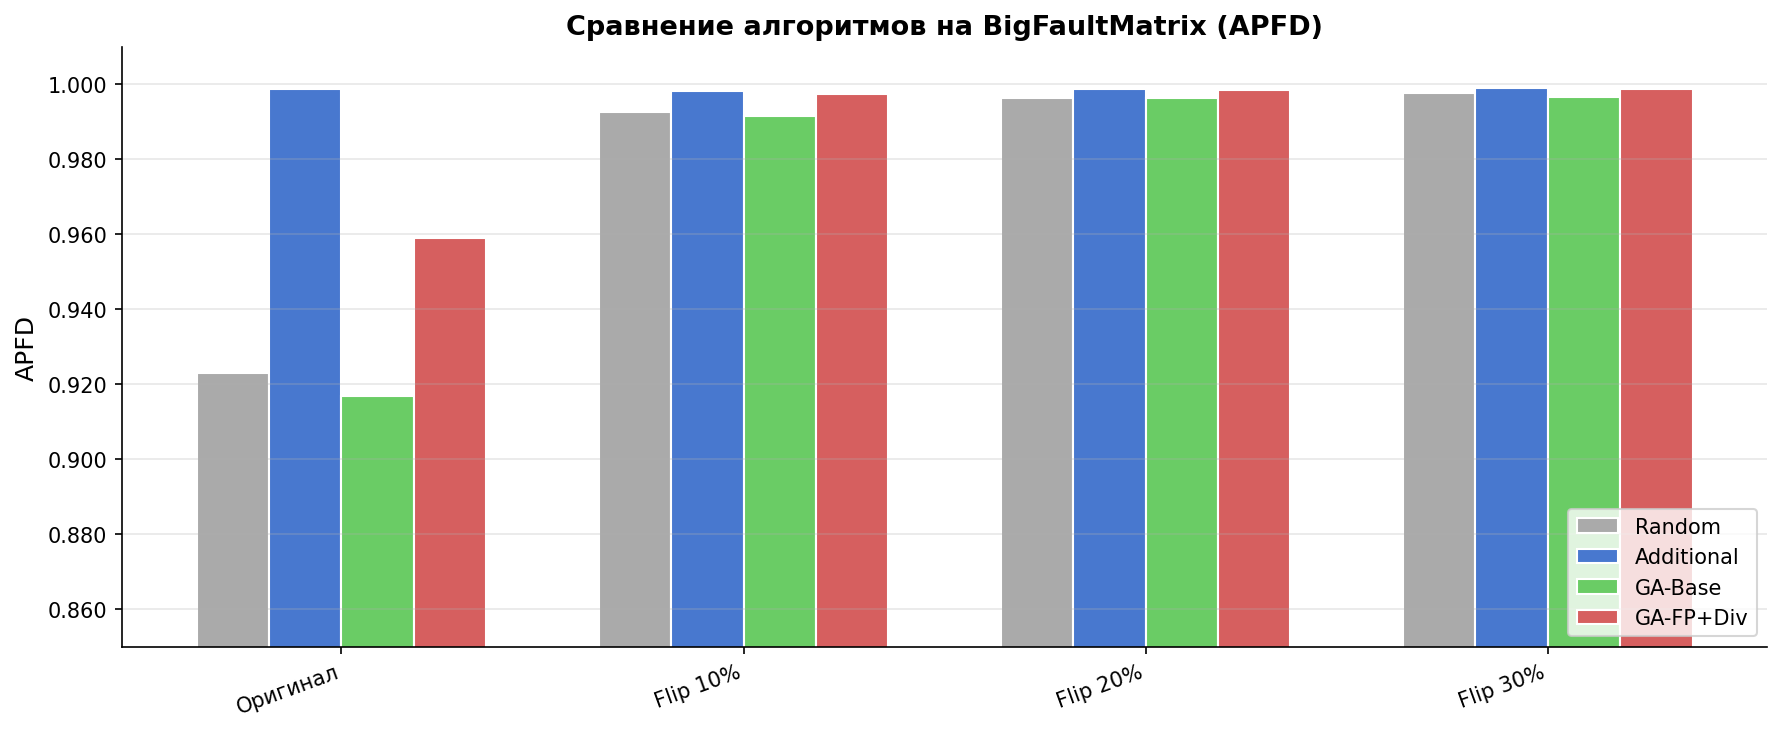
\includegraphics[width=\textwidth]{my_folder/images/bfm_apfd.png}
\caption{Сравнение алгоритмов на BigFaultMatrix по метрике APFD}
\label{fig:bfm}
\end{figure}

На данном наборе данных алгоритм Additional показывает наилучшие результаты во всех четырёх вариациях. 
Это объясняется структурой BigFaultMatrix: покрытие тестов непосредственно соответствует обнаружению 
дефектов, что делает жадную стратегию близкой к оптимальной. Генетические алгоритмы уступают Additional,
поскольку сигнал вероятности дефектов в данном формате слаб.

\section{Результаты на Defects4J} \label{ch6:sec4}

Результаты эксперимента на проектах Defects4J приведены в 
таблице~\ref{tab:d4j} и на рисунке~\ref{fig:d4j}.


\begin{table}[h]
\caption{Результаты на проектах Defects4J (APFD)}
\label{tab:d4j}
\begin{tabularx}{\textwidth}{|X|c|c|c|c|}
\hline
Проект & Random & Additional & GA-Base & GA-FP+Div \\
\hline
Jsoup/93            & 0{,}9115 & 0{,}9811 & 0{,}9936 & \textbf{0{,}9993} \\
Csv/16              & 0{,}9915 & 0{,}9958 & 0{,}9925 & \textbf{0{,}9982} \\
JacksonDatabind/112 & 0{,}8945 & 0{,}8803 & 0{,}8697 & \textbf{0{,}9163} \\
Time/27             & 0{,}9876 & \textbf{0{,}9965} & 0{,}9885 & 0{,}9928 \\
Codec/18            & 0{,}9373 & 0{,}9749 & 0{,}9782 & \textbf{0{,}9950} \\
JacksonCore/26      & 0{,}8643 & \textbf{0{,}9623} & 0{,}8854 & 0{,}9480 \\
Lang/65             & 0{,}9342 & 0{,}9842 & 0{,}9674 & \textbf{0{,}9997} \\
\hline
\end{tabularx}
\end{table}

\begin{figure}[h]
\centering
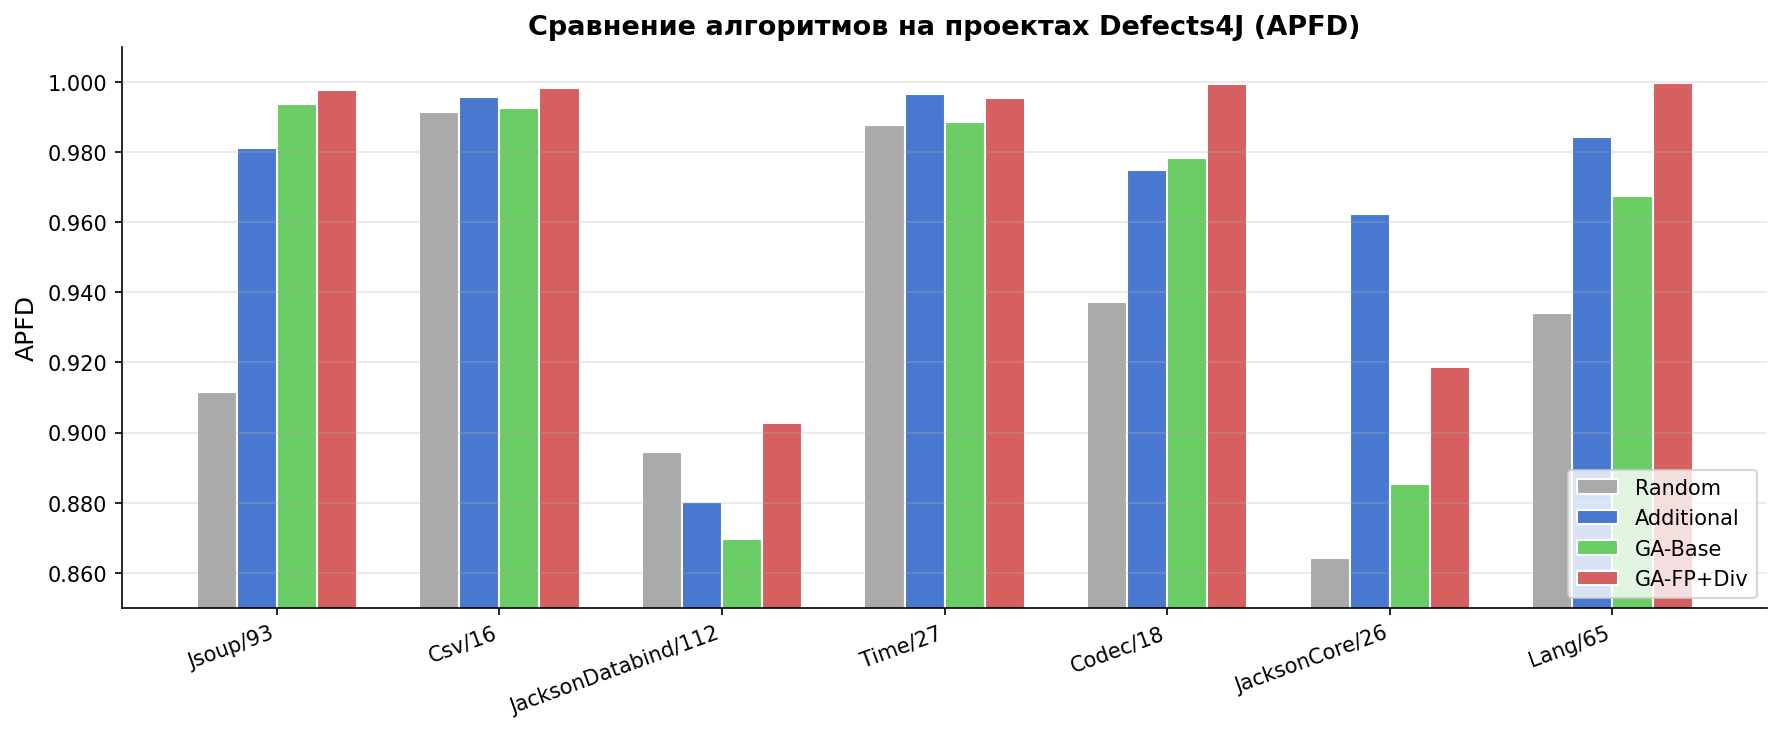
\includegraphics[width=\textwidth]{my_folder/images/defects4j_apfd.png}
\caption{Сравнение алгоритмов на проектах Defects4J по метрике APFD}
\label{fig:d4j}
\end{figure}

\newpage
\section{Анализ результатов} \label{ch6:sec5}

На проектах Defects4J алгоритм GA-FP+Div показывает наилучшие результаты на 5 из 7 проектов. 
На проектах Time/27 и JacksonCore/26 лучшим оказывается Additional. 
Это объясняется малым числом методов с ненулевой вероятностью дефектов по данным CIA-анализа: для 
Time/27 и JacksonCore/26 CIA предоставляет слабый сигнал, что снижает вклад компоненты вероятности 
дефектов в фитнесс-функцию.

На проектах с богатыми CIA-данными (Codec/18, Lang/65, Jsoup/93) преимущество GA-FP+Div наиболее выражено. 
Например, на Codec/18 GA-FP+Div достигает APFD = 0{,}9994, превосходя Additional (0{,}9749) на 2{,}5 
процентных пункта.

Алгоритм GA-Base уступает GA-FP+Div на всех проектах Defects4J, что подтверждает эффективность 
добавления компонент вероятности дефектов и структурного разнообразия в фитнесс-функцию.

Таким образом, GA-FP+Div демонстрирует устойчивое преимущество над базовым генетическим алгоритмом, 
а его эффективность относительно жадного алгоритма определяется качеством CIA-данных для конкретного проекта.   
	        	 % Глава 3
	\ContinueChapterEnd % завершить размещение глав <<подряд>>

	\chapter*{Заключение}
\addcontentsline{toc}{chapter}{Заключение}

В настоящей работе разработан и исследован алгоритм приоритизации тестовых случаев GA-FP+Div, 
представляющий собой генетический алгоритм с улучшенной многокомпонентной фитнесс-функцией. 
Фитнесс-функция учитывает три нормализованных критерия: покрытие кода, вероятность дефектов на основе 
CIA-анализа и структурное разнообразие тестов по расстоянию Жаккара.

В ходе работы получены следующие результаты:

\begin{enumerate}
    \item Проведён анализ существующих методов приоритизации тестовых случаев, выявлены ограничения жадных 
    и эволюционных подходов, обоснована необходимость многокритериальной фитнесс-функции.

    \item Разработана фитнесс-функция, объединяющая покрытие кода, вероятность дефектов и структурное 
    разнообразие тестов. Реализованы операторы OX-кроссовера, адаптивной мутации и элитизма.

    \item Выполнена программная реализация на языке Java с поддержкой загрузки данных в форматах 
    BigFaultMatrix и Defects4J, а также сохранением результатов в форматах CSV и JSON.

    \item Проведён сравнительный эксперимент на наборе данных BigFaultMatrix (4 вариации) и 7 проектах 
    Defects4J. Алгоритм GA-FP+Div показал наилучшие результаты на 5 из 7 проектов Defects4J, 
    превзойдя базовый генетический алгоритм на всех проектах.

    \item Установлено что эффективность GA-FP+Div определяется качеством CIA-данных: на проектах с 
    богатым CIA-анализом (Codec/18, Lang/65) преимущество алгоритма наиболее выражено.
\end{enumerate}

Направления дальнейших исследований включают: автоматический подбор весов фитнесс-функции методами 
настройки гиперпараметров; расширение бенчмарка за счёт дополнительных проектов Defects4J; исследование 
влияния параметра $k$ на качество приоритизации.        	 % Заключение

	%%% Не мянять - Do not modify
%%
%%
\clearpage                                  % В том числе гарантирует, что список литературы в оглавлении будет с правильным номером страницы
%\hypersetup{ urlcolor=black }               % Ссылки делаем чёрными
%\providecommand*{\BibDash}{}                % В стилях ugost2008 отключаем использование тире как разделителя 
\urlstyle{rm}                               % ссылки URL обычным шрифтом
\ifdefmacro{\microtypesetup}{\microtypesetup{protrusion=false}}{} % не рекомендуется применять пакет микротипографики к автоматически генерируемому списку литературы
%\newcommand{\fullbibtitle}{Список литературы} % (ГОСТ Р 7.0.11-2011, 4)
%\insertbibliofull  
%\noindent
%\begin{group}
\chapter*{Список использованных источников}	
\begin{enumerate}[1. ]
    \item Paygude P., Joshi S.~D., Joshi M. Fault Aware Test Case 
    Prioritization in Regression Testing using Genetic Algorithm~// 
    International Journal of Emerging Trends in Engineering Research. 
    --- 2020. --- Vol.~8, No.~5. --- P.~2112--2117. --- 
    DOI:~10.30534/ijeter/2020/104852020.

    \item Mahdieh M., Mirian-Hosseinabadi S.-H., Etemadi K., 
    Bohlouli M. Incorporating Fault-Proneness Estimations into 
    Coverage-Based Test Case Prioritization~// 
    Information and Software Technology. --- 2021. --- Vol.~133. --- 
    P.~106483. --- DOI:~10.1016/j.infsof.2021.106483.

    \item Elbaum S., Malishevsky A.~G., Rothermel G. Test Case 
    Prioritization: A Family of Empirical Studies~// 
    IEEE Transactions on Software Engineering. --- 2002. --- 
    Vol.~28, No.~2. --- P.~159--182. --- 
    DOI:~10.1109/32.988497.

    \item Руденко~М.~А. tcp-methods: репозиторий данных для 
    приоритизации тестовых случаев~// GitHub. --- URL: 
    https://github.com/oneren38/tcp-methods (дата обращения: 
    08.04.2026).

    \item dathpo. Test Case Prioritisation --- Genetic Algorithm: 
    BigFaultMatrix~// GitHub. --- URL: 
    https://github.com/dathpo/Test\_Case\_Prioritisation\_-\_Genetic\_Algorithm 
    (дата обращения: 08.04.2026).
\end{enumerate}

\label{references}
\addcontentsline{toc}{chapter}{Список использованных источников}	% в оглавление 
% \printbibliography[env=SSTfirst]                         % Подключаем Bib-базы
%\ifdefmacro{\microtypesetup}{\microtypesetup{protrusion=true}}{}
%\urlstyle{tt}                               % возвращаем установки шрифта ссылок URL
%\hypersetup{ urlcolor={urlcolor} }          % Восстанавливаем цвет ссылок



%\urlstyle{rm}                               % ссылки URL обычным шрифтом
%\ifdefmacro{\microtypesetup}{\microtypesetup{protrusion=false}}{} % не рекомендуется применять пакет микротипографики к автоматически генерируемому списку литературы
%\insertbibliofull                           % Подключаем Bib-базы
%\ifdefmacro{\microtypesetup}{\microtypesetup{protrusion=true}}{}
%\urlstyle{tt}                               % возвращаем установки шрифта ссылок URL
		     % Список литературы

	% Здесь можно поместить список иллюстративного материала

	\appendix % не редактировать / keep unmodified


	\chapter{Программный код\label{appendix-extra-examples}}							% 

\begin{lstlisting}[language=Java, breaklines=true]
package com.tcp.algorithm;

import com.tcp.model.TestCase;
import java.util.*;


/**
 * базовый жадный алгоритм
 * на каждом шаге выбирает тест, покрывающий наибольшее количество
 */

public class AdditionalPrioritizer implements Prioritizer {

    @Override
    public List<TestCase> prioritize(List<TestCase> testPool) {
        List<TestCase> result = new ArrayList<>();
        Set<String> coveredMethods = new HashSet<>();
        //копия пула, чтобы не модифицировать исходный список
        List<TestCase> remaining = new ArrayList<>(testPool);

        while (!remaining.isEmpty()) {
            TestCase bestTest = null;
            int maxNewCoverage = -1;

            //поиск теста с максимальным новым покрытием
            for (TestCase test : remaining) {
                int newCount = 0;
                for (String method : test.getCoveredMethods()) {
                    if (!coveredMethods.contains(method)) {
                        newCount++;
                    }
                }

                if (newCount > maxNewCoverage) {
                    maxNewCoverage = newCount;
                    bestTest = test;
                } else if (newCount == maxNewCoverage && bestTest != null) {
                    //если покрытие одинаковое берем тест с большей fault proneness
                    if (test.getFaultProneness() > bestTest.getFaultProneness()) {
                        bestTest = test;
                    }
                }
            }
            //fallback: если все оставшиеся тесты не покрывают ничего нового
            if (bestTest == null) {
                bestTest = remaining.get(0);
            }

            result.add(bestTest);
            remaining.remove(bestTest);
            coveredMethods.addAll(bestTest.getCoveredMethods());

        }
        return result;
    }

    @Override
    public String getName() {
        return "Additional";
    }

}
\end{lstlisting}


\begin{lstlisting}[language=Java, breaklines=true]
package com.tcp.algorithm;

import com.tcp.fitness.GaFitnessFunction;
import com.tcp.metric.ApfdCalculator;
import com.tcp.model.TestCase;

import java.util.*;

/**
 * Генетический алгоритм приоритизации тестов.
 *
 * Поддерживает два режима фитнесс-функции:
 *   1. Прямой APFD -- если переданы testToFaults и totalFaults (как в статье Paygude et al.)
 *   2. GaFitnessFunction -- взвешенная сумма coverage + faultProneness + diversity
 *
 * Операторы:
 *   инициализация: случайное перемешивание
 *   селекция: турнирная (tournament selection)
 *   кроссовер: OX (Order Crossover)
 *   мутация: адаптивное число swap = sqrt(n)
 *   элитизм: лучшая особь переходит без изменений
 */
public class GeneticPrioritizer implements Prioritizer {

    private static final int TOURNAMENT_SIZE = 3;

    private final int populationSize;
    private final int generations;
    private final double crossoverRate;
    private final double mutationRate;
    private final GaFitnessFunction fitnessFunction; // null если используется APFD-режим
    private final Map<String, Set<String>> testToFaults; // null если используется GaFitnessFunction
    private final int totalFaults;
    private final Random rng = new Random(42);

    // Конструктор для режима GaFitnessFunction (coverage + faultProneness + diversity)
    public GeneticPrioritizer(int populationSize, int generations,
                              double crossoverRate, double mutationRate,
                              GaFitnessFunction fitnessFunction) {
        this(populationSize, generations, crossoverRate, mutationRate, fitnessFunction, null, 0);
    }

    // Конструктор для режима прямого APFD (как в статье Paygude et al.)
    public GeneticPrioritizer(int populationSize, int generations,
                              double crossoverRate, double mutationRate,
                              GaFitnessFunction fitnessFunction,
                              Map<String, Set<String>> testToFaults,
                              int totalFaults) {
        this.populationSize = populationSize;
        this.generations = generations;
        this.crossoverRate = crossoverRate;
        this.mutationRate = mutationRate;
        this.fitnessFunction = fitnessFunction;
        this.testToFaults = testToFaults;
        this.totalFaults = totalFaults;
    }

    // Выбирает режим фитнесса: прямой APFD или GaFitnessFunction
    private double fitness(List<TestCase> seq) {
        if (testToFaults != null && totalFaults > 0)
            return ApfdCalculator.calculate(seq, testToFaults, totalFaults);
        return fitnessFunction.calculateFitness(seq);
    }

    @Override
    public List<TestCase> prioritize(List<TestCase> testPool) {
        if (testPool.isEmpty()) return new ArrayList<>();

        // адаптивная интенсивность мутации: sqrt(n) swap
        final int mutationIntensity = Math.max(1, (int) Math.sqrt(testPool.size()));

        List<List<TestCase>> population = initPopulation(testPool);
        double[] fit = evalAll(population);

        int bestIdx = argmax(fit);
        List<TestCase> bestEver = new ArrayList<>(population.get(bestIdx));
        double bestFitness = fit[bestIdx];

        for (int gen = 0; gen < generations; gen++) {
            List<List<TestCase>> next = new ArrayList<>(populationSize);
            double[] nextFit = new double[populationSize];

            // элитизм
            next.add(new ArrayList<>(bestEver));
            nextFit[0] = bestFitness;

            while (next.size() < populationSize) {
                List<TestCase> child1 = new ArrayList<>(tournament(population, fit));
                List<TestCase> child2 = new ArrayList<>(tournament(population, fit));

                boolean crossed = false;
                if (rng.nextDouble() < crossoverRate) {
                    oxCrossover(child1, child2);
                    crossed = true;
                }

                boolean mutated1 = false, mutated2 = false;
                if (rng.nextDouble() < mutationRate) { mutate(child1, mutationIntensity); mutated1 = true; }
                if (rng.nextDouble() < mutationRate) { mutate(child2, mutationIntensity); mutated2 = true; }

                int i = next.size();
                next.add(child1);
                nextFit[i] = (crossed || mutated1)
                        ? fitness(child1)
                        : fit[indexOf(population, child1)];

                if (next.size() < populationSize) {
                    int j = next.size();
                    next.add(child2);
                    nextFit[j] = (crossed || mutated2)
                            ? fitness(child2)
                            : fit[indexOf(population, child2)];
                }
            }

            population = next;
            fit = nextFit;

            int idx = argmax(fit);
            if (fit[idx] > bestFitness) {
                bestFitness = fit[idx];
                bestEver = new ArrayList<>(population.get(idx));
            }
        }

        return bestEver;
    }

    private List<List<TestCase>> initPopulation(List<TestCase> pool) {
        List<List<TestCase>> pop = new ArrayList<>(populationSize);
        for (int i = 0; i < populationSize; i++) {
            List<TestCase> ind = new ArrayList<>(pool);
            Collections.shuffle(ind, rng);
            pop.add(ind);
        }
        return pop;
    }

    private double[] evalAll(List<List<TestCase>> population) {
        double[] f = new double[population.size()];
        for (int i = 0; i < population.size(); i++)
            f[i] = fitness(population.get(i));
        return f;
    }

    private List<TestCase> tournament(List<List<TestCase>> population, double[] fit) {
        int best = rng.nextInt(population.size());
        for (int i = 1; i < TOURNAMENT_SIZE; i++) {
            int candidate = rng.nextInt(population.size());
            if (fit[candidate] > fit[best]) best = candidate;
        }
        return population.get(best);
    }

    /**
     * OX (Order Crossover): сохраняет валидную перестановку.
     * Сегмент [start, end] из p1 копируется в child1,
     * остаток заполняется из p2 в порядке появления. Аналогично для child2.
     */
    private void oxCrossover(List<TestCase> p1, List<TestCase> p2) {
        int size = p1.size();
        if (size < 2) return;

        int start = rng.nextInt(size);
        int end = rng.nextInt(size);
        if (start > end) { int tmp = start; start = end; end = tmp; }
        if (start == end) end = Math.min(end + 1, size - 1);

        List<TestCase> c1 = buildOxChild(p1, p2, start, end);
        List<TestCase> c2 = buildOxChild(p2, p1, start, end);
        p1.clear(); p1.addAll(c1);
        p2.clear(); p2.addAll(c2);
    }

    private List<TestCase> buildOxChild(List<TestCase> donor, List<TestCase> filler, int start, int end) {
        int size = donor.size();
        List<TestCase> child = new ArrayList<>(Collections.nCopies(size, null));
        Set<String> inSegment = new HashSet<>();

        for (int i = start; i <= end; i++) {
            child.set(i, donor.get(i));
            inSegment.add(donor.get(i).getId());
        }

        Queue<TestCase> rest = new ArrayDeque<>();
        for (TestCase t : filler)
            if (!inSegment.contains(t.getId())) rest.add(t);

        for (int i = 0; i < size; i++)
            if (child.get(i) == null) child.set(i, rest.poll());

        return child;
    }

    private void mutate(List<TestCase> ind, int intensity) {
        for (int k = 0; k < intensity; k++)
            Collections.swap(ind, rng.nextInt(ind.size()), rng.nextInt(ind.size()));
    }

    private int argmax(double[] arr) {
        int best = 0;
        for (int i = 1; i < arr.length; i++)
            if (arr[i] > arr[best]) best = i;
        return best;
    }

    private int indexOf(List<List<TestCase>> population, List<TestCase> ind) {
        for (int i = 0; i < population.size(); i++)
            if (population.get(i) == ind) return i;
        return 0;
    }

    @Override
    public String getName() { return "GeneticPrioritizer"; }
}
\end{lstlisting}

\begin{lstlisting}[language=Java, breaklines=true]
package com.tcp.algorithm;

import com.tcp.model.TestCase;
import java.util.List;

/*
интерфейс для всех алгоритмов приоритизации
позволяет единообразно вызывать любые стратегии
 */
public interface Prioritizer {
    /**
     * основной метод
     * принимает неупорядоченный пул тестов и возвращает список, отсортированный по приоритету
     *
     * @param testPool  - исходный список тестов
     * @return упорядоченный список тестов
     */
    List<TestCase> prioritize(List<TestCase> testPool);

    /**
     * возвращает название алгоритма для логирования и отчетов
     * @return имя метода приоритизации
     */
    String getName();

}
\end{lstlisting}

\begin{lstlisting}[language=Java, breaklines=true]
package com.tcp.algorithm;

import com.tcp.model.TestCase;

import java.util.*;

/**
 * Random Search -- случайная перестановка тестов.
 * Используется как baseline для сравнения с оптимизационными алгоритмами.
 *
 * Для воспроизводимости результатов используется фиксированный seed.
 * APFD усредняется по нескольким прогонам в Main.
 */
public class RandomPrioritizer implements Prioritizer {

    private final Random rng;

    // seed для воспроизводимости
    public RandomPrioritizer(long seed) {
        this.rng = new Random(seed);
    }

    @Override
    public List<TestCase> prioritize(List<TestCase> testPool) {
        List<TestCase> result = new ArrayList<>(testPool);
        Collections.shuffle(result, rng);
        return result;
    }

    @Override
    public String getName() { return "Random"; }
}

\end{lstlisting}

\begin{lstlisting}[language=Java, breaklines=true]
    package com.tcp.data;

import com.tcp.model.TestCase;

import java.io.*;
import java.util.*;
import java.util.stream.Collectors;

public class DataLoader {

    public static class FaultMatrixData {
        public final List<TestCase> tests;
        public final Map<String, Set<String>> testToFaults;
        public final int totalFaults;

        public FaultMatrixData(List<TestCase> tests, Map<String, Set<String>> testToFaults, int totalFaults) {
            this.tests = tests;
            this.testToFaults = testToFaults;
            this.totalFaults = totalFaults;
        }
    }

    // --- BigFaultMatrix: testId,0,1,0,... ---

    public static FaultMatrixData loadFaultMatrix(String filePath) throws Exception {
        List<TestCase> tests = new ArrayList<>();
        Map<String, Set<String>> testToFaults = new HashMap<>();
        int totalFaults = -1;

        for (String line : readLines(filePath)) {
            String[] parts = line.split(",");
            if (parts.length < 2) continue;
            if (totalFaults == -1) totalFaults = parts.length - 1;

            String testId = parts[0].trim();
            Set<String> killed = new HashSet<>();
            for (int i = 1; i < parts.length; i++)
                if ("1".equals(parts[i].trim())) killed.add("F" + (i - 1));

            double fp = totalFaults > 0 ? (double) killed.size() / totalFaults : 0.0;
            tests.add(new TestCase(testId, killed, fp, 100.0));
            testToFaults.put(testId, killed);
        }

        return new FaultMatrixData(tests, testToFaults, Math.max(totalFaults, 0));
    }

    public static FaultMatrixData createVariation(FaultMatrixData original, double flipRatio, long seed) {
        Random rng = new Random(seed);
        List<TestCase> newTests = new ArrayList<>();
        Map<String, Set<String>> newMap = new HashMap<>();

        for (TestCase t : original.tests) {
            Set<String> faults = new HashSet<>(original.testToFaults.get(t.getId()));
            for (int f = 0; f < original.totalFaults; f++) {
                if (rng.nextDouble() < flipRatio) {
                    String id = "F" + f;
                    if (!faults.add(id)) faults.remove(id);
                }
            }
            double fp = original.totalFaults > 0 ? (double) faults.size() / original.totalFaults : 0.0;
            newTests.add(new TestCase(t.getId(), faults, fp, 100.0));
            newMap.put(t.getId(), faults);
        }

        return new FaultMatrixData(newTests, newMap, original.totalFaults);
    }

    // --- Defects4J / tcp-methods ---
    // Struktura papki projectPath:
    //   coverage/matrix.csv          -- zagolovok: test,method1,...; stroki: testId,0,1,...
    //   mutants/kill.csv             -- MutantNo,[FAIL|TIME|EXC|LIVE|UNCOV]
    //   mutants/testMap.csv          -- TestNo,TestName,Runtime
    //   mutants/covMap.csv           -- TestNo,MutantNo
    //   cia/impact_probabilities.csv -- owner,method,descriptor,roc,fwd,impact

    public static FaultMatrixData loadDefects4JData(String projectPath) throws Exception {
        List<TestCase> tests = loadCoverage(projectPath + "/coverage/matrix.csv");
        Map<String, Set<String>> testToFaults = loadKills(
                projectPath + "/mutants/kill.csv",
                projectPath + "/mutants/testMap.csv",
                projectPath + "/mutants/covMap.csv",
                tests);
        tests = applyImpact(tests, projectPath + "/cia/impact_probabilities.csv");

        int totalFaults = (int) testToFaults.values().stream().flatMap(Set::stream).distinct().count();
        System.out.printf("  Tests: %d, mutants: %d%n", tests.size(), totalFaults);
        return new FaultMatrixData(tests, testToFaults, totalFaults);
    }

    private static List<TestCase> loadCoverage(String path) throws Exception {
        List<TestCase> tests = new ArrayList<>();
        List<String> methods = new ArrayList<>();

        try (BufferedReader br = new BufferedReader(new FileReader(new File(path)))) {
            String line;
            boolean header = true;
            while ((line = br.readLine()) != null) {
                line = line.trim();
                if (line.isEmpty()) continue;
                String[] parts = splitCsv(line);
                if (header) {
                    // первая строка - заголовок с именами методов
                    for (int i = 1; i < parts.length; i++)
                        methods.add(parts[i].replace("\"", "").trim());
                    header = false;
                    continue;
                }
                Set<String> covered = new HashSet<>();
                for (int i = 1; i < parts.length && i - 1 < methods.size(); i++)
                    if ("1".equals(parts[i].trim())) covered.add(methods.get(i - 1));
                tests.add(new TestCase(parts[0].trim(), covered, 0.0, 100.0));
            }
        }
        return tests;
    }

    private static Map<String, Set<String>> loadKills(String killPath, String testMapPath,
                                                      String covMapPath, List<TestCase> tests) throws Exception {
        Map<String, Set<String>> result = new HashMap<>();
        for (TestCase t : tests) result.put(t.getId(), new HashSet<>());

        // kill.csv: MutantNo -> status (FAIL/TIME/EXC = killed)
        Set<String> killed = new HashSet<>();
        for (String line : readLines(killPath)) {
            String[] p = line.split(",");
            if (p.length < 2) continue;
            String status = p[1].trim();
            if (status.equals("FAIL") || status.equals("TIME") || status.equals("EXC"))
                killed.add(p[0].trim());
        }

        // testMap.csv: TestNo -> TestName (className only, no method)
        Map<String, String> testNoToName = new HashMap<>();
        for (String line : readLines(testMapPath)) {
            String[] p = line.split(",");
            if (p.length < 2) continue;
            testNoToName.put(p[0].trim(), p[1].trim());
        }

        // coverage keys look like "org.jsoup.FormElementTest#methodName"
        // testMap has only "org.jsoup.FormElementTest" (class name, no method)
        // build index: className -> list of full testIds from coverage
        Map<String, List<String>> classToIds = new HashMap<>();
        for (String testId : result.keySet()) {
            String cls = testId.contains("#") ? testId.substring(0, testId.indexOf('#')) : testId;
            classToIds.computeIfAbsent(cls, k -> new ArrayList<>()).add(testId);
        }

        // covMap.csv: TestNo,MutantNo - assign killed mutants to tests
        for (String line : readLines(covMapPath)) {
            String[] p = line.split(",");
            if (p.length < 2) continue;
            String testNo = p[0].trim(), mutantNo = p[1].trim();
            if (!killed.contains(mutantNo)) continue;
            String className = testNoToName.get(testNo);
            if (className == null) continue;
            for (String testId : classToIds.getOrDefault(className, Collections.emptyList()))
                result.get(testId).add("M" + mutantNo);
        }

        return result;
    }

    private static List<TestCase> applyImpact(List<TestCase> tests, String path) throws Exception {
        if (!new File(path).exists()) return tests;

        // Нормализуем ключи CIA: org/jsoup/nodes/FormElement,<init>,... -> org.jsoup.nodes.FormElement#init
        Map<String, Double> scores = new HashMap<>();
        for (String line : readLines(path)) {
            String[] p = splitCsv(line);
            if (p.length < 6) continue;
            try {
                String className = p[0].trim().replace('/', '.');
                // убираем угловые скобки: <init> -> init, <clinit> -> clinit
                String methodName = p[1].trim().replace("<", "").replace(">", "");
                String key = className + "#" + methodName;
                double score = Double.parseDouble(p[5].trim());
                scores.merge(key, score, Math::max);
            } catch (NumberFormatException ignored) {}
        }

        // Нормализуем ключи coverage до того же формата:
        // "org.jsoup.parser$Parser#Parser(org.jsoup.parser.TreeBuilder):24" -> "org.jsoup.parser.Parser#Parser"
        return tests.stream().map(t -> {
            double sum = 0.0; int count = 0;
            for (String m : t.getCoveredMethods()) {
                String key = normalizeCoverageKey(m);
                if (scores.containsKey(key)) { sum += scores.get(key); count++; }
            }
            return new TestCase(t.getId(), t.getCoveredMethods(),
                    count > 0 ? sum / count : 0.0, t.getExecutionTimeMs());
        }).collect(Collectors.toList());
    }

    // "org.jsoup.parser$Parser#Parser(org.jsoup.parser.TreeBuilder):24" -> "org.jsoup.parser.Parser#Parser"
    private static String normalizeCoverageKey(String raw) {
        String s = raw.replaceAll(":\\d+$", "");   // убираем :24
        int paren = s.indexOf('(');
        if (paren >= 0) s = s.substring(0, paren); // убираем параметры
        return s.replace('$', '.');                 // $ -> . для вложенных классов
    }


    // --- Synthetic data ---

    /**
     * Генерирует синтетические данные с независимым риском и покрытием.
     *
     * Тесты делятся на три группы чтобы GA-FP+Div имел реальное преимущество:
     *   (30%): большое покрытие, мало фолтов -- жадный выбирает их первыми.
     *   (20%): малое покрытие, высокий риск и много ключевых фолтов.
     *   Обычные (50%): покрытие и фолты пропорциональны density.
     */
    public static FaultMatrixData generateSynthetic(int numTests, int numFaults, double density) {
        List<TestCase> tests = new ArrayList<>();
        Map<String, Set<String>> map = new HashMap<>();
        Random rng = new Random(42);

        // первые 40% фолтов считаются "рискованными"
        int riskFaults = (int)(numFaults * 0.4);

        for (int t = 0; t < numTests; t++) {
            Set<String> faults = new HashSet<>();
            double fp;
            int execTime = 50 + rng.nextInt(150);
            double roll = rng.nextDouble();

            if (roll < 0.30) {
                // "Ловушка": много обычных фолтов, но не рискованных -- низкий риск
                for (int f = riskFaults; f < numFaults; f++)
                    if (rng.nextDouble() < density * 2.5) faults.add("F" + f);
                fp = 0.05 + rng.nextDouble() * 0.05;

            } else if (roll < 0.50) {
                // "Жемчужина": мало покрытия, но попадает в рискованные фолты
                for (int f = 0; f < riskFaults; f++)
                    if (rng.nextDouble() < density * 1.5) faults.add("F" + f);
                fp = 0.6 + rng.nextDouble() * 0.4;

            } else {
                // Обычный тест
                for (int f = 0; f < numFaults; f++)
                    if (rng.nextDouble() < density) faults.add("F" + f);
                fp = numFaults > 0 ? (double) faults.size() / numFaults : 0.0;
            }

            TestCase tc = new TestCase("T" + t, faults, fp, execTime);
            tests.add(tc);
            map.put(tc.getId(), new HashSet<>(faults));
        }

        return new FaultMatrixData(tests, map, numFaults);
    }

    // --- Utils ---

    // Read file line by line, skip empty lines and header (first line)
    private static List<String> readLines(String path) throws Exception {
        List<String> lines = new ArrayList<>();
        File f = new File(path);
        if (!f.exists()) return lines;
        try (BufferedReader br = new BufferedReader(new FileReader(f))) {
            String line;
            boolean header = true;
            while ((line = br.readLine()) != null) {
                line = line.trim();
                if (line.isEmpty()) continue;
                if (header) { header = false; continue; }
                lines.add(line);
            }
        }
        return lines;
    }

    // Split CSV line respecting commas inside quotes
    private static String[] splitCsv(String line) {
        List<String> tokens = new ArrayList<>();
        StringBuilder sb = new StringBuilder();
        boolean inQuotes = false;
        for (char c : line.toCharArray()) {
            if (c == '"') inQuotes = !inQuotes;
            else if (c == ',' && !inQuotes) { tokens.add(sb.toString()); sb.setLength(0); }
            else sb.append(c);
        }
        tokens.add(sb.toString());
        return tokens.toArray(new String[0]);
    }
}
\end{lstlisting}

\begin{lstlisting}[language=Java, breaklines=true]
package com.tcp.fitness;

import com.tcp.model.TestCase;

import java.util.HashSet;
import java.util.List;
import java.util.Set;

/**
 * Фитнесс-функция для генетического алгоритма.
 *
 * Оценивает качество порядка тестов по трём компонентам, каждая в [0, 1]:
 *   coverage -- доля покрытых уникальных методов от всех в пуле
 *   faultProneness -- средний риск первых TOP_K тестов
 *   diversity -- среднее расстояние Жаккара между соседними парами в топ-TOP_K
 *
 * Итоговый фитнесс = взвешенная сумма трёх компонент (веса задаются в конструкторе).
 */
public class GaFitnessFunction {

    // число тестов в начале последовательности, учитываемых для risk и diversity
    private static final int TOP_K = 10;

    private final double weightCoverage;
    private final double weightFaultProneness;
    private final double weightDiversity;

    public GaFitnessFunction(double weightCoverage, double weightFaultProneness, double weightDiversity) {
        this.weightCoverage = weightCoverage;
        this.weightFaultProneness = weightFaultProneness;
        this.weightDiversity = weightDiversity;
    }

    // Вычисляет фитнесс последовательности.
    // totalMethods вычисляется каждый раз из пула - безопасно при смене проектов.
    public double calculateFitness(List<TestCase> seq) {
        if (seq.isEmpty()) return 0.0;

        Set<String> all = new HashSet<>();
        for (TestCase t : seq) all.addAll(t.getCoveredMethods());
        int totalMethods = Math.max(all.size(), 1);

        return weightCoverage      * coverage(seq, totalMethods)
                + weightFaultProneness * faultProneness(seq)
                + weightDiversity      * diversity(seq);
    }

    // Доля уникальных покрытых методов от totalMethods
    private double coverage(List<TestCase> seq, int totalMethods) {
        Set<String> covered = new HashSet<>();
        for (TestCase t : seq) covered.addAll(t.getCoveredMethods());
        return (double) covered.size() / totalMethods;
    }

    // Средняя fault-proneness первых TOP_K тестов
    private double faultProneness(List<TestCase> seq) {
        int k = Math.min(seq.size(), TOP_K);
        double sum = 0.0;
        for (int i = 0; i < k; i++) sum += seq.get(i).getFaultProneness();
        return sum / k;
    }

    // Среднее расстояние Жаккара между соседними парами в топ-TOP_K
    private double diversity(List<TestCase> seq) {
        int k = Math.min(seq.size(), TOP_K);
        if (k < 2) return 0.0;
        double sum = 0.0;
        for (int i = 0; i < k - 1; i++)
            sum += jaccard(seq.get(i).getCoveredMethods(), seq.get(i + 1).getCoveredMethods());
        return sum / (k - 1);
    }

    // Расстояние Жаккара: 0 = одинаковые, 1 = полностью разные множества
    private double jaccard(Set<String> a, Set<String> b) {
        if (a.isEmpty() && b.isEmpty()) return 0.0;
        if (a.isEmpty() || b.isEmpty()) return 1.0;

        // считаем пересечение без создания нового множества
        int intersection = 0;
        for (String s : a) if (b.contains(s)) intersection++;
        int union = a.size() + b.size() - intersection;

        return 1.0 - (double) intersection / union;
    }
}
\end{lstlisting}

\begin{lstlisting}[language=Java, breaklines=true]
package com.tcp.metric;

import com.tcp.model.TestCase;

import java.util.*;

/**
 * Метрика APFD (Average Percentage of Faults Detected).
 * Оценивает скорость обнаружения дефектов: чем ближе к 1, тем раньше находятся мутанты.
 *
 * Формула: APFD = 1 - sumTF / (n * m) + 1 / (2n)
 *   n -- число тестов
 *   m -- число мутантов
 *   sumTF -- сумма позиций первых тестов, обнаруживших каждый мутант
 */
public class ApfdCalculator {

    public static double calculate(List<TestCase> orderedTests,
                                   Map<String, Set<String>> testToMutants,
                                   int totalMutants) {
        int n = orderedTests.size();
        int m = totalMutants;
        if (n == 0 || m == 0) return 0.0;

        Set<String> detected = new HashSet<>();
        double sumTF = 0.0;

        for (int i = 0; i < n; i++) {
            for (String mutant : testToMutants.getOrDefault(orderedTests.get(i).getId(), Collections.emptySet())) {
                if (detected.add(mutant)) sumTF += (i + 1);
            }
        }

        return 1.0 - sumTF / ((double) n * m) + 1.0 / (2.0 * n);
    }
}
\end{lstlisting}

\begin{lstlisting}[language=Java, breaklines=true]
package com.tcp.metric;

import com.tcp.model.TestCase;

import java.util.*;

/**
 * Метрика APFDc (APFD with Cost) - APFD с учётом времени выполнения тестов.
 *
 * В отличие от APFD, взвешивает обнаружение мутантов по кумулятивному времени:
 * мутант, найденный быстрым тестом в начале, ценится выше чем найденный медленным в конце.
 *
 * Формула: APFDc = sum(totalTime - cumTime_i + execTime_i / 2) / (totalTime * m)
 *   totalTime -- суммарное время всех тестов
 *   cumTime_i -- кумулятивное время до конца теста i
 *   m -- число мутантов
 */
public class ApfdCostCalculator {

    public static double calculateWithCost(List<TestCase> orderedTests,
                                           Map<String, Set<String>> testToMutants,
                                           int totalMutants) {
        if (orderedTests.isEmpty() || totalMutants == 0) return 0.0;

        double totalTime = orderedTests.stream().mapToDouble(TestCase::getExecutionTimeMs).sum();
        Set<String> detected = new HashSet<>();
        double weightedSum = 0.0;
        double cumTime = 0.0;

        for (TestCase test : orderedTests) {
            cumTime += test.getExecutionTimeMs();
            for (String mutant : testToMutants.getOrDefault(test.getId(), Collections.emptySet())) {
                if (detected.add(mutant))
                    weightedSum += totalTime - cumTime + test.getExecutionTimeMs() / 2.0;
            }
        }

        return weightedSum / (totalTime * totalMutants);
    }
}
\end{lstlisting}

\begin{lstlisting}[language=Java, breaklines=true]
    package com.tcp;

import com.tcp.algorithm.AdditionalPrioritizer;
import com.tcp.algorithm.GeneticPrioritizer;
import com.tcp.algorithm.Prioritizer;
import com.tcp.algorithm.RandomPrioritizer;
import com.tcp.data.DataLoader;
import com.tcp.data.DataLoader.FaultMatrixData;
import com.tcp.fitness.GaFitnessFunction;
import com.tcp.metric.ApfdCalculator;
import com.tcp.metric.ApfdCostCalculator;
import com.tcp.model.TestCase;

import java.io.*;
import java.time.LocalDateTime;
import java.time.format.DateTimeFormatter;
import java.util.*;

/**
 * Точка входа бенчмарка приоритизации регрессионных тестов.
 *
 * Алгоритмы:
 *   Random      -- случайная перестановка (среднее по 5 прогонам)
 *   Additional  -- жадный baseline по покрытию
 *   GA-Base     -- ГА только с покрытием (coverage weight = 1.0)
 *   GA-FP+Div   -- ГА с fault-proneness и диверсификацией (0.4 / 0.4 / 0.2)
 *
 * Метрики: APFD, APFDc
 * Результаты сохраняются в results/results.csv и results/results.json
 */
public class Main {

    private static final String BFM_PATH    = "data/bigfaultmatrix/bigfaultmatrix.txt";
    private static final String RESULTS_DIR = "results";
    private static final String CSV_PATH    = RESULTS_DIR + "/results.csv";
    private static final String JSON_PATH   = RESULTS_DIR + "/results.json";
    private static final int    RANDOM_RUNS = 5;

    private static final List<String> DEFAULT_PROJECTS = List.of(
            "Jsoup/93", "Csv/16", "JacksonDatabind/112",
            "Time/27", "Codec/18", "JacksonCore/26", "Lang/65"
    );

    // Хранит все результаты текущей сессии для записи в файлы
    private static final List<ResultRow> allResults = new ArrayList<>();

    public static void main(String[] args) {
        initResultsDir();
        Scanner sc = new Scanner(System.in);
        System.out.println("=== TCP Benchmark ===");

        while (true) {
            System.out.println("\n1. BigFaultMatrix (4 вариации)");
            System.out.println("2. Defects4J");
            System.out.println("3. Синтетические данные");
            System.out.println("4. Все Defects4J проекты");
            System.out.println("0. Выход");
            System.out.print("Выбор: ");
            String choice = sc.nextLine().trim();

            switch (choice) {
                case "1": runBigFaultMatrix(); break;
                case "2":
                    System.out.print("Путь к проекту (например data/raw/Jsoup/93): ");
                    String path = sc.nextLine().trim();
                    runBenchmark(path, loadOrNull(() -> DataLoader.loadDefects4JData(path)));
                    break;
                case "3": runBenchmark("synthetic", runSynthetic(sc)); break;
                case "4": runAllProjects(sc); break;
                case "0":
                    saveResults();
                    sc.close();
                    return;
                default: System.out.println("Введите 0-4.");
            }

            System.out.print("\nНажмите Enter...");
            sc.nextLine();
        }
    }

    // --- Прогоны ---

    private static void runBigFaultMatrix() {
        FaultMatrixData original = loadOrNull(() -> DataLoader.loadFaultMatrix(BFM_PATH));
        if (original == null) return;

        System.out.println("\n=== BigFaultMatrix: 4 вариации ===");

        String[] labels = { "BFM-original", "BFM-flip10", "BFM-flip20", "BFM-flip30" };
        double[] flips  = { 0.0, 0.1, 0.2, 0.3 };
        long[]   seeds  = { 0L,  1L,  2L,  3L  };

        System.out.printf("%n%-22s | %-8s | %-8s | %-8s | %-8s | %s%n",
                "Вариация", "Random", "Additional", "GA-Base", "GA-FP+Div", "Лучший");
        System.out.println("-".repeat(82));

        for (int v = 0; v < 4; v++) {
            FaultMatrixData data = (v == 0)
                    ? original
                    : DataLoader.createVariation(original, flips[v], seeds[v]);

            int gens = adaptiveGens(data.tests.size());
            Map<String, double[]> metrics = collectMetrics(data, gens);

            double[] rnd = metrics.get("Random");
            double[] add = metrics.get("Additional");
            double[] gab = metrics.get("GA-Base");
            double[] gaf = metrics.get("GA-FP+Div");

            String best = bestName(new double[]{rnd[0], add[0], gab[0], gaf[0]},
                    new String[]{"Random", "Additional", "GA-Base", "GA-FP+Div"});

            System.out.printf("%-22s | %-8.4f | %-8.4f | %-8.4f | %-8.4f | %s%n",
                    labels[v], rnd[0], add[0], gab[0], gaf[0], best);

            allResults.add(new ResultRow(labels[v], data.tests.size(), data.totalFaults,
                    rnd[0], rnd[1], add[0], add[1], gab[0], gab[1], gaf[0], gaf[1]));
        }
        System.out.println("-".repeat(82));
    }

    private static FaultMatrixData runSynthetic(Scanner sc) {
        int tests   = readInt(sc,    "Тестов (100): ",   100);
        int faults  = readInt(sc,    "Фолтов (50): ",     50);
        double dens = readDouble(sc, "Плотность (0.1): ", 0.1);
        return DataLoader.generateSynthetic(tests, faults, dens);
    }

    private static void runBenchmark(String label, FaultMatrixData data) {
        if (data == null || data.tests.isEmpty() || data.totalFaults == 0) {
            System.err.println("Нет данных для бенчмарка.");
            return;
        }

        int gens = adaptiveGens(data.tests.size());
        System.out.printf("  Поколений ГА: %d%n", gens);

        Map<String, double[]> metrics = collectMetrics(data, gens);
        printResults(metrics);

        double[] rnd = metrics.get("Random");
        double[] add = metrics.get("Additional");
        double[] gab = metrics.get("GA-Base");
        double[] gaf = metrics.get("GA-FP+Div");

        allResults.add(new ResultRow(label, data.tests.size(), data.totalFaults,
                rnd[0], rnd[1], add[0], add[1], gab[0], gab[1], gaf[0], gaf[1]));
    }

    private static void runAllProjects(Scanner sc) {
        System.out.print("Базовый путь к данным (например data/raw): ");
        String base = sc.nextLine().trim();

        System.out.println("\n=== ПАКЕТНЫЙ ЗАПУСК ===");
        System.out.printf("%-25s | %-8s | %-8s | %-8s | %-8s | %s%n",
                "Проект", "Random", "Additional", "GA-Base", "GA-FP+Div", "Лучший");
        System.out.println("-".repeat(82));

        for (String project : DEFAULT_PROJECTS) {
            FaultMatrixData data = loadOrNull(() -> DataLoader.loadDefects4JData(base + "/" + project));

            if (data == null || data.tests.isEmpty() || data.totalFaults == 0) {
                System.out.printf("%-25s | ПРОПУЩЕН%n", project);
                continue;
            }

            int gens = adaptiveGens(data.tests.size());
            Map<String, double[]> metrics = collectMetrics(data, gens);

            double[] rnd = metrics.get("Random");
            double[] add = metrics.get("Additional");
            double[] gab = metrics.get("GA-Base");
            double[] gaf = metrics.get("GA-FP+Div");

            String best = bestName(new double[]{rnd[0], add[0], gab[0], gaf[0]},
                    new String[]{"Random", "Additional", "GA-Base", "GA-FP+Div"});

            System.out.printf("%-25s | %-8.4f | %-8.4f | %-8.4f | %-8.4f | %s%n",
                    project, rnd[0], add[0], gab[0], gaf[0], best);

            allResults.add(new ResultRow(project, data.tests.size(), data.totalFaults,
                    rnd[0], rnd[1], add[0], add[1], gab[0], gab[1], gaf[0], gaf[1]));
        }
        System.out.println("-".repeat(82));
    }

    // --- Сбор метрик ---

    // Запускает все алгоритмы и возвращает Map: algorithmName -> [apfd, apfdc]
    private static Map<String, double[]> collectMetrics(FaultMatrixData data, int gens) {
        Map<String, double[]> result = new LinkedHashMap<>();

        // Random: среднее по RANDOM_RUNS прогонам
        double sumApfd = 0, sumApfdc = 0;
        for (int r = 0; r < RANDOM_RUNS; r++) {
            List<TestCase> ordered = new RandomPrioritizer(r).prioritize(new ArrayList<>(data.tests));
            sumApfd  += ApfdCalculator.calculate(ordered, data.testToFaults, data.totalFaults);
            sumApfdc += ApfdCostCalculator.calculateWithCost(ordered, data.testToFaults, data.totalFaults);
        }
        result.put("Random", new double[]{ sumApfd / RANDOM_RUNS, sumApfdc / RANDOM_RUNS });

        // Additional, GA-Base, GA-FP+Div
        List<String> names = List.of("Additional", "GA-Base", "GA-FP+Div");
        List<Prioritizer> algorithms = new ArrayList<>();
        algorithms.add(new AdditionalPrioritizer());
        algorithms.add(new GeneticPrioritizer(100, gens, 0.8, 0.2, new GaFitnessFunction(1.0, 0.0, 0.0)));
        algorithms.add(new GeneticPrioritizer(100, gens, 0.8, 0.2, new GaFitnessFunction(0.4, 0.4, 0.2)));

        for (int i = 0; i < algorithms.size(); i++) {
            List<TestCase> ordered = algorithms.get(i).prioritize(new ArrayList<>(data.tests));
            double apfd  = ApfdCalculator.calculate(ordered, data.testToFaults, data.totalFaults);
            double apfdc = ApfdCostCalculator.calculateWithCost(ordered, data.testToFaults, data.totalFaults);
            result.put(names.get(i), new double[]{ apfd, apfdc });
            // сохраняем упорядоченный список для вывода топ-3
            orderedResults.put(names.get(i), ordered);
        }
        // Random топ-3: берём первый прогон
        orderedResults.put("Random",
                new RandomPrioritizer(0).prioritize(new ArrayList<>(data.tests)));

        return result;
    }

    // хранит упорядоченные списки тестов для вывода топ-3
    private static final Map<String, List<TestCase>> orderedResults = new LinkedHashMap<>();

    private static void printResults(Map<String, double[]> metrics) {
        System.out.println("\n--- РЕЗУЛЬТАТЫ ---");
        System.out.printf("%-20s | %-8s | %-8s%n", "Алгоритм", "APFD", "APFDc");
        System.out.println("-".repeat(42));

        String bestName = null; double bestApfd = -1;
        for (Map.Entry<String, double[]> e : metrics.entrySet()) {
            System.out.printf("%-20s | %-8.4f | %-8.4f%n", e.getKey(), e.getValue()[0], e.getValue()[1]);
            if (e.getValue()[0] > bestApfd) { bestApfd = e.getValue()[0]; bestName = e.getKey(); }
        }
        System.out.println("-".repeat(42));
        System.out.printf("Лучший: %s (APFD = %.4f)%n", bestName, bestApfd);

        // Топ-3 тестов для каждого алгоритма
        System.out.println("\n--- ТОП-3 ТЕСТОВ ---");
        for (Map.Entry<String, List<TestCase>> e : orderedResults.entrySet()) {
            System.out.printf("%n%s:%n", e.getKey());
            System.out.printf("  %-12s | %-8s | %-10s%n", "Тест", "Risk", "Coverage");
            System.out.println("  " + "-".repeat(36));
            List<TestCase> ordered = e.getValue();
            for (int i = 0; i < Math.min(3, ordered.size()); i++) {
                TestCase t = ordered.get(i);
                System.out.printf("  %-12s | %-8.3f | %d%n",
                        t.getId(), t.getFaultProneness(),
                        t.getCoveredMethods().size());
            }
        }
        orderedResults.clear();
    }

    // --- Сохранение результатов ---

    private static void saveResults() {
        if (allResults.isEmpty()) return;
        try {
            new File(RESULTS_DIR).mkdirs();
            saveCsv();
            saveJson();
            System.out.println("\nРезультаты сохранены:");
            System.out.println("  CSV:  " + CSV_PATH);
            System.out.println("  JSON: " + JSON_PATH);
        } catch (Exception e) {
            System.err.println("Ошибка сохранения: " + e.getMessage());
        }
    }

    private static void saveCsv() throws Exception {
        // Используем ; как разделитель - Excel в русской локали ожидает именно его
        // sep= в первой строке подсказывает Excel какой разделитель использован
        boolean exists = new File(CSV_PATH).exists();
        try (PrintWriter pw = new PrintWriter(
                new OutputStreamWriter(new FileOutputStream(CSV_PATH, true), "UTF-8"))) {
            if (!exists) {
                pw.println("sep=;");  // директива для Excel - автоматически выберет разделитель
                pw.println("timestamp;dataset;tests;faults;" +
                        "random_apfd;random_apfdc;" +
                        "additional_apfd;additional_apfdc;" +
                        "gabase_apfd;gabase_apfdc;" +
                        "gafpdiv_apfd;gafpdiv_apfdc");
            }
            String ts = LocalDateTime.now().format(DateTimeFormatter.ofPattern("yyyy-MM-dd HH:mm:ss"));
            for (ResultRow r : allResults)
                pw.printf("%s;%s;%d;%d;%.4f;%.4f;%.4f;%.4f;%.4f;%.4f;%.4f;%.4f%n",
                        ts, r.dataset, r.tests, r.faults,
                        r.randomApfd, r.randomApfdc,
                        r.addApfd, r.addApfdc,
                        r.gaBaseApfd, r.gaBaseApfdc,
                        r.gaFpApfd, r.gaFpApfdc);
        }
    }

    private static void saveJson() throws Exception {
        String ts = LocalDateTime.now().format(DateTimeFormatter.ofPattern("yyyy-MM-dd HH:mm:ss"));
        StringBuilder sb = new StringBuilder("[\n");
        for (int i = 0; i < allResults.size(); i++) {
            ResultRow r = allResults.get(i);
            sb.append("  {\n");
            sb.append(String.format("    \"timestamp\": \"%s\",\n", ts));
            sb.append(String.format("    \"dataset\": \"%s\",\n", r.dataset));
            sb.append(String.format("    \"tests\": %d,\n", r.tests));
            sb.append(String.format("    \"faults\": %d,\n", r.faults));
            sb.append(String.format("    \"Random\":     {\"apfd\": %.4f, \"apfdc\": %.4f},\n", r.randomApfd, r.randomApfdc));
            sb.append(String.format("    \"Additional\": {\"apfd\": %.4f, \"apfdc\": %.4f},\n", r.addApfd, r.addApfdc));
            sb.append(String.format("    \"GA-Base\":    {\"apfd\": %.4f, \"apfdc\": %.4f},\n", r.gaBaseApfd, r.gaBaseApfdc));
            sb.append(String.format("    \"GA-FP+Div\": {\"apfd\": %.4f, \"apfdc\": %.4f}\n", r.gaFpApfd, r.gaFpApfdc));
            sb.append(i < allResults.size() - 1 ? "  },\n" : "  }\n");
        }
        sb.append("]");
        try (PrintWriter pw = new PrintWriter(new FileWriter(JSON_PATH))) {
            pw.print(sb);
        }
    }

    // --- Вспомогательные методы ---

    private static int adaptiveGens(int n) {
        return Math.max(50, (int)(Math.log(n) / Math.log(2)) * 10);
    }

    private static String bestName(double[] apfds, String[] names) {
        int best = 0;
        for (int i = 1; i < apfds.length; i++) if (apfds[i] > apfds[best]) best = i;
        return names[best];
    }

    private static void initResultsDir() {
        new File(RESULTS_DIR).mkdirs();
    }

    private static FaultMatrixData loadOrNull(ThrowingSupplier<FaultMatrixData> supplier) {
        try { return supplier.get(); }
        catch (Exception e) { System.err.println("Ошибка загрузки: " + e.getMessage()); return null; }
    }

    private static int readInt(Scanner sc, String prompt, int defaultVal) {
        System.out.print(prompt);
        String s = sc.nextLine().trim();
        return s.isEmpty() ? defaultVal : Integer.parseInt(s);
    }

    private static double readDouble(Scanner sc, String prompt, double defaultVal) {
        System.out.print(prompt);
        String s = sc.nextLine().trim();
        return s.isEmpty() ? defaultVal : Double.parseDouble(s);
    }

    @FunctionalInterface
    private interface ThrowingSupplier<T> { T get() throws Exception; }

    // --- Модель строки результата ---

    private static class ResultRow {
        final String dataset;
        final int tests, faults;
        final double randomApfd, randomApfdc;
        final double addApfd, addApfdc;
        final double gaBaseApfd, gaBaseApfdc;
        final double gaFpApfd, gaFpApfdc;

        ResultRow(String dataset, int tests, int faults,
                  double randomApfd, double randomApfdc,
                  double addApfd, double addApfdc,
                  double gaBaseApfd, double gaBaseApfdc,
                  double gaFpApfd, double gaFpApfdc) {
            this.dataset = dataset; this.tests = tests; this.faults = faults;
            this.randomApfd = randomApfd; this.randomApfdc = randomApfdc;
            this.addApfd = addApfd; this.addApfdc = addApfdc;
            this.gaBaseApfd = gaBaseApfd; this.gaBaseApfdc = gaBaseApfdc;
            this.gaFpApfd = gaFpApfd; this.gaFpApfdc = gaFpApfdc;
        }
    }
}
\end{lstlisting}			     % Приложение 1

	% \chapter{Программный код\label{appendix-extra-examples}}							% 

\begin{verbatim}
	##LoopStatisticsAlgorithm
package algorithms;

import java.util.ArrayList;
import java.util.Collections;
import java.util.List;

public class LoopStatisticsAlgorithm implements StatisticsAlgorithm {

    @Override
    public String getName() {
        return "Loop-based (Imperative)";
    }

    @Override
    public double min(List<Double> data) {
        if (data.isEmpty()) throw new RuntimeException("Пустая выборка");
        double min = Double.MAX_VALUE;
        for (double x : data) {
            if (x < min) min = x;
        }
        return min;
    }

    @Override
    public double max(List<Double> data) {
        if (data.isEmpty()) throw new RuntimeException("Пустая выборка");
        double max = -Double.MAX_VALUE;
        for (double x : data) {
            if (x > max) max = x;
        }
        return max;
    }

    @Override
    public double mean(List<Double> data) {
        if (data.isEmpty()) throw new RuntimeException("Пустая выборка");
        double sum = 0.0;
        for (double x : data) {
            sum += x;
        }
        return sum / data.size();
    }

    @Override
    public double median(List<Double> data) {
        if (data.isEmpty()) throw new RuntimeException("Пустая выборка");
        List<Double> temp = new ArrayList<>(data);
        Collections.sort(temp);
        int n = temp.size();
        int mid = n / 2;
        if (n % 2 == 0) {
            return (temp.get(mid - 1) + temp.get(mid)) / 2.0;
        } else {
            return temp.get(mid);
        }
    }

    @Override
    public double variance(List<Double> data) {
        if (data.isEmpty()) throw new RuntimeException("Пустая выборка");
        if (data.size() < 2) throw new RuntimeException("Недостаточно данных");
        double m = mean(data);
        double sum = 0.0;
        for (double x : data) {
            sum += (x - m) * (x - m);
        }
        return sum / (data.size() - 1);
    }

    @Override
    public double skewness(List<Double> data) {
        if (data.isEmpty()) throw new RuntimeException("Пустая выборка");
        double m = mean(data);
        double v = variance(data);
        double sum = 0.0;
        for (double x : data) {
            sum += Math.pow(x - m, 3);
        }
        return sum / data.size() / Math.pow(v, 1.5);
    }

    @Override
    public double kurtosis(List<Double> data) {
        int n = data.size();
        if (n < 4) throw new RuntimeException("Недостаточно данных для эксцесса");
        double sum1 = 0.0;
        for (double x : data) sum1 += x;
        double mean = sum1 / n;
        double sx2 = 0.0;
        double sum4 = 0.0;
        for (double x : data) {
            double d = x - mean;
            sx2 += d * d;
            sum4 += d * d * d * d;
        }
        sx2 /= (n - 1);
        if (sx2 == 0.0) throw new RuntimeException("Дисперсия равна нулю");
        double sum4Norm = sum4 / Math.pow(sx2, 2);
        return (n * (n + 1.0) / ((n - 1) * (n - 2) * (n - 3))) * sum4Norm
                - 3.0 * (n - 1) * (n - 1) / ((n - 2) * (n - 3));
    }
	

##StatisticsAlgorithm
package algorithms;

import java.util.List;

public interface StatisticsAlgorithm {

    double min(List<Double> data);

    double max(List<Double> data);

    double mean(List<Double> data);

    double median(List<Double> data);

    double variance(List<Double> data);

    double skewness(List<Double> data);

    double kurtosis(List<Double> data);

    String getName();
}

##StreamStatisticsAlgorithm
package algorithms;

import java.util.ArrayList;
import java.util.Collections;
import java.util.List;

public class StreamStatisticsAlgorithm implements StatisticsAlgorithm {

    @Override
    public String getName() {
        return "Stream-based (Functional)";
    }

    @Override
    public double min(List<Double> data) {
        if (data.isEmpty()) throw new RuntimeException("Пустая выборка");
        return data.stream().mapToDouble(Double::doubleValue).min().orElseThrow();
    }

    @Override
    public double max(List<Double> data) {
        if (data.isEmpty()) throw new RuntimeException("Пустая выборка");
        return data.stream().mapToDouble(Double::doubleValue).max().orElseThrow();
    }

    @Override
    public double mean(List<Double> data) {
        if (data.isEmpty()) throw new RuntimeException("Пустая выборка");
        return data.stream().mapToDouble(Double::doubleValue).average().orElseThrow();
    }

    @Override
    public double median(List<Double> data) {
        if (data.isEmpty()) throw new RuntimeException("Пустая выборка");
        List<Double> temp = new ArrayList<>(data);
        Collections.sort(temp);
        int n = temp.size();
        int mid = n / 2;
        if (n % 2 == 0) {
            return (temp.get(mid - 1) + temp.get(mid)) / 2.0;
        } else {
            return temp.get(mid);
        }
    }

    @Override
    public double variance(List<Double> data) {
        if (data.isEmpty()) throw new RuntimeException("Пустая выборка");
        if (data.size() < 2) throw new RuntimeException("Недостаточно данных");
        double m = mean(data);
        double sum = data.stream()
                .mapToDouble(x -> (x - m) * (x - m))
                .sum();
        return sum / (data.size() - 1);
    }

    @Override
    public double skewness(List<Double> data) {
        if (data.isEmpty()) throw new RuntimeException("Пустая выборка");
        double m = mean(data);
        double v = variance(data);
        double sum = data.stream()
                .mapToDouble(x -> Math.pow(x - m, 3))
                .sum();
        return sum / data.size() / Math.pow(v, 1.5);
    }

    @Override
    public double kurtosis(List<Double> data) {
        int n = data.size();
        if (n < 4) throw new RuntimeException("Недостаточно данных для эксцесса");
        double mean = data.stream().mapToDouble(Double::doubleValue).average().orElseThrow();
        double sx2 = data.stream()
                .mapToDouble(x -> (x - mean) * (x - mean))
                .sum() / (n - 1);
        if (sx2 == 0.0) throw new RuntimeException("Дисперсия равна нулю");
        double sum4 = data.stream()
                .mapToDouble(x -> {
                    double d = x - mean;
                    return d * d * d * d;
                })
                .sum();
        double sum4Norm = sum4 / Math.pow(sx2, 2);
        return (n * (n + 1.0) / ((n - 1) * (n - 2) * (n - 3))) * sum4Norm
                - 3.0 * (n - 1) * (n - 1) / ((n - 2) * (n - 3));
    }


##SampleData
package json;

import java.util.List;

public class SampleData {

    public String sampleType;
    public List<Double> data;
    public double minVal;
    public double maxVal;
    public double meanVal;
    public double stddevVal;

    public SampleData() {
    }

    public SampleData(String sampleType, List<Double> data) {
        this.sampleType = sampleType;
        this.data = data;
    }

    public SampleData withUniformParams(double min, double max) {
        this.minVal = min;
        this.maxVal = max;
        return this;
    }

    public SampleData withNormalParams(double mean, double stddev) {
        this.meanVal = mean;
        this.stddevVal = stddev;
        return this;
    }
}

##ConsoleSample
package samples;

import json.SampleData;

import java.util.ArrayList;
import java.util.List;
import java.util.Scanner;

public class ConsoleSample extends Sample {

    public ConsoleSample() {
        super();
    }

    @Override
    public void generate(int n) {
        if (n <= 0) {
            throw new IllegalArgumentException("Размер выборки должен быть положительным");
        }

        data.clear();
        Scanner scanner = new Scanner(System.in);

        System.out.println("Введите " + n + " чисел выборки (каждое с новой строки):");

        int count = 0;
        while (count < n) {
            if (scanner.hasNextDouble()) {
                double value = scanner.nextDouble();
                data.add(value);
                count++;
            } else {
                String invalid = scanner.next();
                System.out.println("Ошибка ввода. Введите число ещё раз:");
            }
        }
    }

    public void setData(List<Double> values) {
        data.clear();
        data.addAll(values);
    }

    @Override
    protected SampleData createSampleData() {
        return new SampleData("ConsoleSample", new ArrayList<>(data));
    }

    @Override
    protected void restoreFromSampleData(SampleData sampleData) {
    }

    @Override
    public String toString() {
        return String.format("ConsoleSample[size=%d]", data.size());
    }

    @Override
    public boolean equals(Object obj) {
        if (this == obj) return true;
        if (obj == null || getClass() != obj.getClass()) return false;
        ConsoleSample that = (ConsoleSample) obj;
        return data.equals(that.data);
    }

    @Override
    public int hashCode() {
        return data.hashCode();
    }
}

##FileSample
package samples;

import json.SampleData;

import java.util.ArrayList;
import java.util.List;

public class FileSample extends Sample {

    public FileSample() {
        super();
    }

    public FileSample(List<Double> values) {
        super();
        this.data.addAll(values);
    }

    @Override
    public void generate(int n) {
    }

    public void setData(List<Double> values) {
        data.clear();
        data.addAll(values);
    }

    @Override
    protected SampleData createSampleData() {
        return new SampleData("FileSample", new ArrayList<>(data));
    }

    @Override
    protected void restoreFromSampleData(SampleData sampleData) {
    }

    @Override
    public String toString() {
        return String.format("FileSample[size=%d]", data.size());
    }

    @Override
    public boolean equals(Object obj) {
        if (this == obj) return true;
        if (obj == null || getClass() != obj.getClass()) return false;
        FileSample that = (FileSample) obj;
        return data.equals(that.data);
    }

    @Override
    public int hashCode() {
        return data.hashCode();
    }
}

##Main
package samples;

import algorithms.LoopStatisticsAlgorithm;
import algorithms.StreamStatisticsAlgorithm;
import json.*;
import utils.*;
import samples.*;

public class Main {

    public static void main(String[] args) {
        UniformSample uniformSample = null;
        NormalSample normalSample = null;
        FileSample fileSample = null;
        ConsoleSample consoleSample = null;

        while (true) {
           System.out.println("\n=====================================");
            System.out.println("       Статистический калькулятор");
            System.out.println("=====================================");
            System.out.println("1. Ввести выборку вручную");
            System.out.println("2. Создать равномерную выборку");
            System.out.println("3. Создать нормальную выборку");
            System.out.println("4. Загрузить из JSON");
            System.out.println("5. Вывести показатели");
            System.out.println("6. Сохранить в JSON");
            System.out.println("7. Оценка взаимозависимости двух выборок");
            System.out.println("8. Выход");
            System.out.println("=====================================");

            int choice = ReadFunctions.readInt("Выберите пункт меню: ", 0, 10);

            switch (choice) {
                case 0: {
                    System.out.println("\n----ТЕСТИРОВАНИЕ----");
                    System.out.println("Запустите тесты через Maven: mvn test");
                    break;
                }
                case 1: {
                    int n = ReadFunctions.readInt("Введите количество элементов: ", 1, 100000);
                    consoleSample = new ConsoleSample();
                    consoleSample.generate(n);
                    System.out.println("\nВыборка сохранена");
                    break;
                }
                case 2: {
                    int n = ReadFunctions.readInt("Размер выборки: ", 1, 100000);
                    double a = ReadFunctions.readDouble("Минимум: ");
                    double b = ReadFunctions.readDouble("Максимум: ", a, Double.MAX_VALUE);
                    uniformSample = new UniformSample(a, b);
                    uniformSample.generate(n);
                    System.out.println("Равномерная выборка создана, n = " + n);
                    break;
                }
                case 3: {
                    int n = ReadFunctions.readInt("Размер выборки: ", 1, 100000);
                    double mean = ReadFunctions.readDouble("Среднее значение: ");
                    double stddev = ReadFunctions.readDouble("Стандартное отклонение: ", 0, Double.MAX_VALUE);
                    normalSample = new NormalSample(mean, stddev);
                    normalSample.generate(n);
                    System.out.println("Нормальная выборка создана, n = " + n);
                    break;
                }
                case 4: {
                    try {
                        String filename = ReadFunctions.readString("Введите имя файла (.json): ");
                        SampleData sampleData = JsonUtils.loadFromJson(filename);

                        switch (sampleData.sampleType) {
                            case "UniformSample":
                                uniformSample = new UniformSample(sampleData.minVal, sampleData.maxVal);
                                uniformSample.loadFromJson(filename);
                                System.out.println("Загружено UniformSample: " + uniformSample.getData().size() + " элементов");
                                break;
                            case "NormalSample":
                                normalSample = new NormalSample(sampleData.meanVal, sampleData.stddevVal);
                                normalSample.loadFromJson(filename);
                                System.out.println("Загружено NormalSample: " + normalSample.getData().size() + " элементов");
                                break;
                            case "FileSample":
                            case "ConsoleSample":
                                fileSample = new FileSample();
                                fileSample.loadFromJson(filename);
                                System.out.println("Загружено: " + fileSample.getData().size() + " элементов");
                                break;
                            default:
                                System.out.println("Неизвестный тип выборки: " + sampleData.sampleType);
                        }
                    } catch (RuntimeException e) {
                        System.out.println("Ошибка: " + e.getMessage());
                    }
                    break;
                }
                case 5: {
                    if (consoleSample != null) {
                        System.out.println("\nВведенная выборка:");
                        consoleSample.showCharact();
                    }
                    if (uniformSample != null) {
                        System.out.println("\nРавномерная выборка:");
                        uniformSample.showCharact();
                    }
                    if (normalSample != null) {
                        System.out.println("\nНормальная выборка:");
                        normalSample.showCharact();
                    }
                    if (fileSample != null) {
                        System.out.println("\nВыборка из файла:");
                        fileSample.showCharact();
                    }
                    break;
                }
                case 6: {
                    int sampleChoice = ReadFunctions.readInt(
                            "\nВыберите выборку для сохранения в JSON: \n1 - Равномерная\n2 - Нормальная\n3 - Из файла\n4 - Введенная\nВведите число: ", 1, 4);

                    Sample selectedSample = pickSample(sampleChoice, uniformSample, normalSample, fileSample, consoleSample);

                    if (selectedSample != null) {
                        try {
                            String filename = ReadFunctions.readString("Введите имя файла (.json): ");
                            selectedSample.saveToJson(filename.endsWith(".json") ? filename : filename + ".json");
                            System.out.println("Выборка сохранена в JSON");
                        } catch (RuntimeException e) {
                            System.out.println("Ошибка: " + e.getMessage());
                        }
                    } else {
                        System.out.println("Сначала создайте выборку");
                    }
                    break;
                }
                case 7: {
                    int a = ReadFunctions.readInt(
                            "Выберите первую выборку:\n1 - Равномерная\n2 - Нормальная\n3 - Из файла\n4 - Введенная\nВыбор: ", 1, 4);
                    int b = ReadFunctions.readInt("Выберите вторую выборку: ", 1, 4);

                    Sample s1 = pickSample(a, uniformSample, normalSample, fileSample, consoleSample);
                    Sample s2 = pickSample(b, uniformSample, normalSample, fileSample, consoleSample);

                    if (s1 == null || s2 == null) {
                        System.out.println("Одна из выборок не существует");
                        break;
                    }
                    try {
                        double r = StatsUtils.correlation(s1, s2);
                        System.out.printf("Коэффициент корреляции Пирсона: %.4f%n", r);
                    } catch (RuntimeException e) {
                        System.out.println("Ошибка: " + e.getMessage());
                    }
                    break;
                }

                case 8: {
                    System.out.println("Выход...");
                    return;
                }
                default:
                    System.out.println("Неверный выбор!");
                    break;
            }
        }
    }

    private static Sample pickSample(int choice, UniformSample uniform, NormalSample normal, FileSample file, ConsoleSample console) {
        return switch (choice) {
            case 1 -> uniform;
            case 2 -> normal;
            case 3 -> file;
            case 4 -> console;
            default -> null;
        };
    }
}

##NormalSample
package samples;

import json.SampleData;

import java.util.ArrayList;
import java.util.List;
import java.util.Random;

public class NormalSample extends Sample {

    private double meanVal;
    private double stddevVal;

    private static final Random random = new Random();

    public NormalSample() {
        super();
        this.meanVal = 0.0;
        this.stddevVal = 1.0;
    }

    public NormalSample(double mean, double stddev) {
        super();
        this.meanVal = mean;
        this.stddevVal = stddev;
    }

    @Override
    public void generate(int n) {
        if (n <= 0) {
            throw new IllegalArgumentException("Размер выборки должен быть положительным");
        }
        if (stddevVal <= 0) {
            throw new IllegalArgumentException("Стандартное отклонение должно быть положительным");
        }

        data.clear();

        if (data instanceof ArrayList) {
            ((ArrayList<Double>) data).ensureCapacity(n);
        }

        for (int i = 0; i < n; i++) {
            double randomValue = meanVal + stddevVal * random.nextGaussian();
            data.add(randomValue);
        }
    }

    @Override
    protected SampleData createSampleData() {
        return new SampleData("NormalSample", new ArrayList<>(data))
                .withNormalParams(meanVal, stddevVal);
    }

    @Override
    protected void restoreFromSampleData(SampleData sampleData) {
        this.meanVal = sampleData.meanVal;
        this.stddevVal = sampleData.stddevVal;
    }

    public double getMeanVal() {
        return meanVal;
    }

    public void setMeanVal(double meanVal) {
        this.meanVal = meanVal;
    }

    public double getStddevVal() {
        return stddevVal;
    }

    public void setStddevVal(double stddevVal) {
        this.stddevVal = stddevVal;
    }

    @Override
    public String toString() {
        return String.format("NormalSample[mean=%.2f, stddev=%.2f, size=%d]",
                meanVal, stddevVal, data.size());
    }

    @Override
    public boolean equals(Object obj) {
        if (this == obj) return true;
        if (obj == null || getClass() != obj.getClass()) return false;
        NormalSample that = (NormalSample) obj;
        return Double.compare(that.meanVal, meanVal) == 0 &&
                Double.compare(that.stddevVal, stddevVal) == 0 &&
                data.equals(that.data);
    }

    @Override
    public int hashCode() {
        int result;
        long temp;
        temp = Double.doubleToLongBits(meanVal);
        result = (int) (temp ^ (temp >>> 32));
        temp = Double.doubleToLongBits(stddevVal);
        result = 31 * result + (int) (temp ^ (temp >>> 32));
        result = 31 * result + data.hashCode();
        return result;
    }
}

##Sample
package samples;

import algorithms.StatisticsAlgorithm;
import algorithms.LoopStatisticsAlgorithm;
import json.SampleData;
import utils.JsonUtils;

import java.io.*;
import java.nio.file.*;
import java.util.*;

public abstract class Sample {

    protected List<Double> data;
    private StatisticsAlgorithm algorithm = new LoopStatisticsAlgorithm();

    public Sample() {
        this.data = new ArrayList<>();
    }

    public Sample(StatisticsAlgorithm algorithm) {
        this.data = new ArrayList<>();
        this.algorithm = algorithm;
    }

    public void setData(List<Double> values){
        this.data.clear();
        this.data.addAll(values);
    }

    public abstract void generate(int n);

    public List<Double> getData() {
        return Collections.unmodifiableList(data);
    }

    public void setAlgorithm(StatisticsAlgorithm algorithm) {
        this.algorithm = algorithm;
    }

    public StatisticsAlgorithm getAlgorithm() {
        return this.algorithm;
    }

    public double min() {
        return algorithm.min(data);
    }

    public double max() {
        return algorithm.max(data);
    }

    public double mean() {
        return algorithm.mean(data);
    }

    public double median() {
        return algorithm.median(data);
    }

    public double variance() {
        return algorithm.variance(data);
    }

    public double skewness() {
        return algorithm.skewness(data);
    }

    public double kurtosis() {
        return algorithm.kurtosis(data);
    }

    public List<Double> quartiles() {
        if (data.isEmpty()) {
            throw new RuntimeException("Пустая выборка");
        }

        List<Double> temp = new ArrayList<>(data);
        Collections.sort(temp);

        int n = temp.size();
        double q1 = getQuantile(temp, 0.25);
        double q2 = median();
        double q3 = getQuantile(temp, 0.75);

        return Arrays.asList(q1, q2, q3);
    }

    private double getQuantile(List<Double> sortedData, double q) {
        int n = sortedData.size();
        double pos = q * (n - 1);
        int index = (int) pos;
        double frac = pos - index;

        if (index + 1 < n) {
            return sortedData.get(index) + frac * (sortedData.get(index + 1) - sortedData.get(index));
        } else {
            return sortedData.get(index);
        }
    }

    public boolean isNormal(double alpha) {
        double jb = jarqueBera();
        double critical;

        if (alpha == 0.10) critical = 4.605;
        else if (alpha == 0.05) critical = 5.991;
        else if (alpha == 0.01) critical = 9.210;
        else throw new RuntimeException("Неподдерживаемый уровень значимости: " + alpha);

        return jb < critical;
    }

    public double jarqueBera() {
        if (data.size() < 3) {
            throw new RuntimeException("Недостаточно данных для теста Jarque-Bera");
        }
        double n = (double) data.size();
        double s = skewness();
        double k = kurtosis();
        return (n / 6.0) * (s * s + (k * k) / 4.0);
    }

    public void saveToFile(String filename) {
        try (BufferedWriter writer = Files.newBufferedWriter(Paths.get(filename))) {
            for (double x : data) {
                writer.write(String.valueOf(x));
                writer.newLine();
            }
        } catch (IOException e) {
            throw new RuntimeException("Не удалось сохранить файл: " + e.getMessage());
        }
    }

    public void loadFromFile(String filename) {
        data.clear();
        try (BufferedReader reader = Files.newBufferedReader(Paths.get(filename))) {
            String line;
            while ((line = reader.readLine()) != null) {
                if (!line.trim().isEmpty()) {
                    data.add(Double.parseDouble(line.trim()));
                }
            }
        } catch (IOException e) {
            throw new RuntimeException("Не удалось загрузить файл: " + e.getMessage());
        }

        if (data.isEmpty()) {
            throw new RuntimeException("Файл пуст или не содержит чисел");
        }
    }

    public void saveToJson(String filename) {
        SampleData sampleData = createSampleData();
        JsonUtils.saveToJson(sampleData, filename);
    }

    public void loadFromJson(String filename) {
        SampleData sampleData = JsonUtils.loadFromJson(filename);
        data.clear();
        data.addAll(sampleData.data);
        restoreFromSampleData(sampleData);
    }

    protected SampleData createSampleData() {
        return new SampleData(this.getClass().getSimpleName(), new ArrayList<>(data));
    }

    protected void restoreFromSampleData(SampleData sampleData) {
    }

    public void showCharact() {
        System.out.println("=======================================");
        System.out.println("  Статистика выборки: " + this.getClass().getSimpleName());
        System.out.println("  Алгоритм: " + algorithm.getName());
        System.out.println("=======================================");
        System.out.println("  Размер выборки: " + data.size());
        System.out.println("---------------------------------------");
        System.out.printf("  Минимум:        %.4f%n", this.min());
        System.out.printf("  Максимум:       %.4f%n", this.max());
        System.out.printf("  Среднее:        %.4f%n", this.mean());
        System.out.printf("  Медиана:        %.4f%n", this.median());
        System.out.println("---------------------------------------");

        List<Double> q = this.quartiles();
        System.out.printf("  Квартиль 0.25:  %.4f%n", q.get(0));
        System.out.printf("  Квартиль 0.50:  %.4f%n", q.get(1));
        System.out.printf("  Квартиль 0.75:  %.4f%n", q.get(2));
        System.out.println("---------------------------------------");

        System.out.printf("  Дисперсия:      %.4f%n", this.variance());
        System.out.printf("  Асимметрия:     %.4f%n", this.skewness());
        System.out.printf("  Эксцесс:        %.4f%n", this.kurtosis());
        System.out.println("("=======================================");

        try {
            double jb = this.jarqueBera();
            boolean isNormal = this.isNormal(0.05);
            System.out.printf("  Тест Jarque-Bera: %.4f%n", jb);
            System.out.println("  Нормальность: " + (isNormal ? "не отвергается" : "отвергается"));
        } catch (Exception e) {
            System.out.println("  Тест на нормальность: невозможно проверить");
        }
        System.out.println("("=======================================");
    }

    @Override
    public String toString() {
        return String.format("%s[size=%d, algorithm=%s]",
                this.getClass().getSimpleName(),
                data.size(),
                algorithm.getName());
    }

    @Override
    public boolean equals(Object obj) {
        if (this == obj) return true;
        if (obj == null || getClass() != obj.getClass()) return false;
        Sample sample = (Sample) obj;
        return data.equals(sample.data);
    }

    @Override
    public int hashCode() {
        return data.hashCode();
    }
}

##UniformSample
package samples;

import json.SampleData;

import java.util.ArrayList;
import java.util.List;

public class UniformSample extends Sample {

    private double minVal;
    private double maxVal;

    public UniformSample() {
        super();
        this.minVal = 0.0;
        this.maxVal = 1.0;
    }

    public UniformSample(double min, double max) {
        super();
        this.minVal = min;
        this.maxVal = max;
    }

    @Override
    public void generate(int n) {
        if (n <= 0) {
            throw new IllegalArgumentException("Размер выборки должен быть положительным");
        }
        if (minVal >= maxVal) {
            throw new IllegalArgumentException("minVal должен быть меньше maxVal");
        }

        data.clear();

        if (data instanceof ArrayList) {
            ((ArrayList<Double>) data).ensureCapacity(n);
        }

        for (int i = 0; i < n; i++) {
            double randomValue = minVal + (maxVal - minVal) * Math.random();
            data.add(randomValue);
        }
    }

    @Override
    protected SampleData createSampleData() {
        return new SampleData("UniformSample", new ArrayList<>(data))
                .withUniformParams(minVal, maxVal);
    }

    @Override
    protected void restoreFromSampleData(SampleData sampleData) {
        this.minVal = sampleData.minVal;
        this.maxVal = sampleData.maxVal;
    }

    public double getMinVal() {
        return minVal;
    }

    public void setMinVal(double minVal) {
        this.minVal = minVal;
    }

    public double getMaxVal() {
        return maxVal;
    }

    public void setMaxVal(double maxVal) {
        this.maxVal = maxVal;
    }

    @Override
    public String toString() {
        return String.format("UniformSample[min=%.2f, max=%.2f, size=%d]",
                minVal, maxVal, data.size());
    }

    @Override
    public boolean equals(Object obj) {
        if (this == obj) return true;
        if (obj == null || getClass() != obj.getClass()) return false;
        UniformSample that = (UniformSample) obj;
        return Double.compare(that.minVal, minVal) == 0 &&
                Double.compare(that.maxVal, maxVal) == 0 &&
                data.equals(that.data);
    }

    @Override
    public int hashCode() {
        int result;
        long temp;
        temp = Double.doubleToLongBits(minVal);
        result = (int) (temp ^ (temp >>> 32));
        temp = Double.doubleToLongBits(maxVal);
        result = 31 * result + (int) (temp ^ (temp >>> 32));
        result = 31 * result + data.hashCode();
        return result;
    }
}

##JsonUtils
package utils;

import com.google.gson.Gson;
import com.google.gson.GsonBuilder;
import com.google.gson.stream.JsonReader;
import json.SampleData;

import java.io.*;
import java.nio.file.*;

public class JsonUtils {

    private static final Gson gson = new GsonBuilder()
            .setPrettyPrinting()
            .create();

    private JsonUtils() {
    }

    public static void saveToJson(SampleData sampleData, String filename) {
        try (BufferedWriter writer = Files.newBufferedWriter(Paths.get(filename))) {
            gson.toJson(sampleData, writer);
        } catch (IOException e) {
            throw new RuntimeException("Не удалось сохранить JSON: " + e.getMessage());
        }
    }

    public static SampleData loadFromJson(String filename) {
        try (BufferedReader reader = Files.newBufferedReader(Paths.get(filename));
             JsonReader jsonReader = new JsonReader(reader)) {
            return gson.fromJson(jsonReader, SampleData.class);
        } catch (IOException e) {
            throw new RuntimeException("Не удалось загрузить JSON: " + e.getMessage());
        }
    }

    public static String toJson(SampleData sampleData) {
        return gson.toJson(sampleData);
    }
}

##ReadFunctions
package utils;

import java.util.Scanner;

public class ReadFunctions {

    private static Scanner scanner = new Scanner(System.in);


    public static Scanner getScanner(){
        return scanner;
    }

    private ReadFunctions() {
    }

    public static int readInt(String prompt, int min, int max) {
        int value;
        while (true) {
            System.out.print(prompt);
            if (scanner.hasNextInt()) {
                value = scanner.nextInt();
                if (value >= min && value <= max) {
                    return value;
                } else {
                    System.out.println("Число должно быть от " + min + " до " + max);
                }
            } else {
                System.out.println("Неверный ввод. Попробуйте еще раз");
                scanner.next();
            }
        }
    }

    public static int readInt(String prompt) {
        return readInt(prompt, Integer.MIN_VALUE, Integer.MAX_VALUE);
    }

    public static double readDouble(String prompt, double min, double max) {
        double value;
        while (true) {
            System.out.print(prompt);
            if (scanner.hasNextDouble()) {
                value = scanner.nextDouble();
                if (value >= min && value <= max) {
                    return value;
                } else {
                    System.out.println("Число должно быть от " + min + " до " + max);
                }
            } else {
                System.out.println("Неверный ввод. Попробуйте еще раз");
                scanner.next();
            }
        }
    }

    public static double readDouble(String prompt) {
        return readDouble(prompt, Double.NEGATIVE_INFINITY, Double.POSITIVE_INFINITY);
    }

    public static String readString(String prompt) {
        System.out.print(prompt);
        return scanner.next();
    }
}

##StatsUtils
package utils;

import samples.Sample;

import java.util.List;

public class StatsUtils {

    private StatsUtils() {
    }

    public static double correlation(Sample a, Sample b) {
        List<Double> x = a.getData();
        List<Double> y = b.getData();

        if (x.size() != y.size()) {
            throw new RuntimeException("Выборки должны быть одного размера");
        }
        if (x.size() < 2) {
            throw new RuntimeException("Недостаточно данных");
        }

        double meanX = a.mean();
        double meanY = b.mean();

        double num = 0.0;
        double sx = 0.0;
        double sy = 0.0;

        for (int i = 0; i < x.size(); i++) {
            double dx = x.get(i) - meanX;
            double dy = y.get(i) - meanY;
            num += dx * dy;
            sx += dx * dx;
            sy += dy * dy;
        }

        if (sx == 0.0 || sy == 0.0) {
            throw new RuntimeException("Нулевая дисперсия одной из выборок");
        }

        return num / Math.sqrt(sx * sy);
    }
}

##LoopStatisticsAlgorithmTest
package algorithm;

import algorithms.LoopStatisticsAlgorithm;
import algorithms.StatisticsAlgorithm;
import algorithms.StreamStatisticsAlgorithm;
import org.junit.jupiter.api.Test;
import org.junit.jupiter.api.DisplayName;
import org.junit.jupiter.params.ParameterizedTest;
import org.junit.jupiter.params.provider.ValueSource;
import org.mockito.Mockito;

import static org.junit.jupiter.api.Assertions.*;
import static org.junit.jupiter.api.Assumptions.*;
import static org.hamcrest.MatcherAssert.assertThat;
import static org.hamcrest.Matchers.*;
import static org.mockito.Mockito.*;

import java.util.Arrays;
import java.util.Collections;
import java.util.List;
import java.util.ArrayList;

import static org.mockito.ArgumentMatchers.anyList;


@DisplayName("Тестирование LoopStatisticsAlgorithm")
public class LoopStatisticsAlgorithmTest {
    private final StatisticsAlgorithm loopAlgorithm = new LoopStatisticsAlgorithm();
    private final StatisticsAlgorithm streamAlgorithm = new StreamStatisticsAlgorithm();

    //ГРАНИЧНЫЕ ЗНАЧЕНИЯ (BoundaryValue)
    @Test
    @DisplayName("Граничное значение: пустой список должен выбрасывать исключение")
    void testMinEmptyList_BoundaryValue() {
        //граничное значение 0 элементов
        assertThrows(RuntimeException.class, () -> loopAlgorithm.min(Collections.emptyList()));
    }

    @Test
    @DisplayName("Граничное значение: один элемент")
    void testMinSingleElement_BoundaryValue() {
        //граничное значение 1 элемент
        List<Double> data = Collections.singletonList(5.0);
        double result = loopAlgorithm.min(data);
        assertEquals(5.0, result, 0.0001);
    }

    @Test
    @DisplayName("Граничное значение: 1 элемент для дисперсии должен выбрасывать исключение")
    void testVarianceOneElement_BoundaryValue() {
        //меньше минимального: 1 элемент
        List<Double> data = Collections.singletonList(5.0);
        assertThrows(RuntimeException.class, () -> loopAlgorithm.variance(data));
    }

    @Test
    @DisplayName("Граничное значение: 3 элемента для эксцесса должен выбрасывать исключение")
    void testKurtosisThreeElements_BoundaryValue() {
        //меньше минимального: 3 элемента
        List<Double> data = Arrays.asList(1.0, 2.0, 3.0);
        assertThrows(RuntimeException.class, () -> loopAlgorithm.kurtosis(data));
    }

    // КЛАССЫ ЭКВИВАЛЕНТНОСТИ (Equivalence Partitioning)
    @ParameterizedTest
    @ValueSource(doubles = {1.0, 5.5, 100.0})
    @DisplayName("Класс эквивалентности: положительные числа")
    void testMeanPositiveNumbers_EquivalenceClass(double value) {
        List<Double> data = Arrays.asList(value, value, value);
        double result = loopAlgorithm.mean(data);
        assertThat(result, is(closeTo(value, 0.0001)));
    }

    @ParameterizedTest
    @ValueSource(doubles = {-1.0, -5.5, -100.0})
    @DisplayName("Класс эквивалентности: отрицательные числа")
    void testMeanNegativeNumbers_EquivalenceClass(double value) {
        List<Double> data = Arrays.asList(value, value, value);
        double result = loopAlgorithm.mean(data);
        assertThat(result, is(closeTo(value, 0.0001)));
    }

    @Test
    @DisplayName("Медиана: нечетное количество (3 элемента)")
    void testMedianOddCount() {
        List<Double> data = Arrays.asList(1.0, 2.0, 3.0);
        assertEquals(2.0, loopAlgorithm.median(data), 0.0001);
    }

    @Test
    @DisplayName("Медиана: четное количество (4 элемента)")
    void testMedianEvenCount() {
        List<Double> data = Arrays.asList(1.0, 2.0, 3.0, 4.0);
        assertEquals(2.5, loopAlgorithm.median(data), 0.0001);
    }

    //ПОКРЫТИЕ ОПЕРАТОРОВ (Statement Testing)
    @Test
    @DisplayName("Покрытие операторов: все методы должны выполниться")
    void testAllMethodExecute_StatementCoverage() {
        List<Double> data = Arrays.asList(1.0, 2.0, 3.0, 4.0, 5.0);

        //каждый метод выполнится хотя бы один раз
        double min = loopAlgorithm.min(data);
        double max = loopAlgorithm.max(data);
        double mean = loopAlgorithm.mean(data);
        double median = loopAlgorithm.median(data);
        double variance = loopAlgorithm.variance(data);
        double skewness = loopAlgorithm.skewness(data);
        double kurtosis = loopAlgorithm.kurtosis(data);
        String name = loopAlgorithm.getName();

        //проверка, что все значения получены
        assertAll("Все методы выполнены успешно",
                () -> assertNotNull(min),
                () -> assertNotNull(max),
                () -> assertNotNull(mean),
                () -> assertNotNull(median),
                () -> assertNotNull(variance),
                () -> assertNotNull(skewness),
                () -> assertNotNull(kurtosis),
                () -> assertNotNull(name));
    }

    //ПОКРЫТИЕ ВЕТВЛЕНИЙ (Branch Testing)
    @Test
    @DisplayName("Покрытие ветвлений: медиана для нечетного количества (else)")
    void testMedianOddCount_BranchCoverage() {
        //n%2!=0
        List<Double> data = Arrays.asList(1.0, 3.0, 2.0);
        double result = loopAlgorithm.median(data);
        assertEquals(2.0, result, 0.0001);
    }

    @Test
    @DisplayName("Покрытие ветвлений: медиана для нечетного количества (if)")
    void testMedianEvenCount_BranchCoverage() {
        //n%2==0
        List<Double> data = Arrays.asList(1.0, 3.0, 2.0, 4.0);
        double result = loopAlgorithm.median(data);
        assertEquals(2.5, result, 0.0001);
    }

    @Test
    @DisplayName("Покрытие ветвлений: isEmpty() - true/false")
    void testIsEmpty_BranchCoverage() {
        //пустой список
        assertThrows(RuntimeException.class, () -> loopAlgorithm.min(Collections.emptyList()));

        //заполненный список
        List<Double> data = Collections.singletonList(1.0);
        assertDoesNotThrow(() -> loopAlgorithm.min(data));
    }

    //СРАВНЕНИЕ АЛГОРИТМОВ
    @Test
    @DisplayName("Сравнение алгоритмов: Loop и Stream должны давать одинаковые результаты")
    void testLoopVsStreamAlgorithmComparison() {
        List<Double> data = Arrays.asList(1.0, 5.0, 3.0, 9.0, 2.0, 7.0, 4.0);

        double loopMin = loopAlgorithm.min(data);
        double streamMin = streamAlgorithm.min(data);
        assertEquals(loopMin, streamMin, 0.0001, "min должен совпадать");

        double loopMax = loopAlgorithm.max(data);
        double streamMax = streamAlgorithm.max(data);
        assertEquals(loopMax, streamMax, 0.0001, "max должен совпадать");

        double loopMean = loopAlgorithm.mean(data);
        double streamMean = streamAlgorithm.mean(data);
        assertEquals(loopMean, streamMean, 0.0001, "mean должен совпадать");

        double loopMedian = loopAlgorithm.median(data);
        double streamMedian = streamAlgorithm.median(data);
        assertEquals(loopMedian, streamMedian, 0.0001, "median должен совпадать");

        double loopVariance = loopAlgorithm.variance(data);
        double streamVariance = streamAlgorithm.variance(data);
        assertEquals(loopVariance, streamVariance, 0.0001, "variance должен совпадать");
    }

    @ParameterizedTest
    @ValueSource(ints = {5, 10, 20, 50})
    @DisplayName("Сравнение алгоритмов на разных размерах выборки")
    void testLoopVsStreamVariousSizes(int size) {
        List<Double> data = new ArrayList<>();
        for (int i = 0; i < size; i++) {
            data.add((double) i);
        }

        double loopResult = loopAlgorithm.mean(data);
        double streamResult = streamAlgorithm.mean(data);

        assertEquals(loopResult, streamResult, 0.0001,
                "Результаты должны совпадать для размера" + size);
    }

    //ASSUMPTIONS
    @Test
    @DisplayName("Assumption: тест имеет смысл только для положительных размеров")
    void testWithAssumptionOnSize() {
        List<Double> data = Arrays.asList(1.0, 2.0, 3.0);

        //предположение: тест имеет смысл только если данных больше 2
        assumeTrue(data.size() > 2, "Требуется минимум 3 элемента");

        double variance = loopAlgorithm.variance(data);
        assertTrue(variance >= 0, "Дисперсия не может быть отрицательной");
    }

    @Test
    @DisplayName("Assumption: пропускаем тест если выборка пустая")
    void testWithAssumptionOnEmptyList() {
        List<Double> data = Arrays.asList(1.0, 2.0, 3.0, 4.0, 5.0);

        //предположение: данные не должны быть пустыми
        assumeFalse(data.isEmpty(), "Данные не должны быть пустыми");

        double mean = loopAlgorithm.mean(data);
        assertThat(mean, is(greaterThan(0.0)));
    }

    //MOCKS
    @Test
    @DisplayName("Mock: создание мока StatisticsAlgorithm")
    void testMockStatisticsAlgorithm() {
        //создаем пустой мок
        StatisticsAlgorithm mockAlg = Mockito.mock(StatisticsAlgorithm.class);

        //проверка, что мок создан
        assertNotNull(mockAlg);

        //вызов метода (возврат default для double-0.0)
        double result = mockAlg.mean(Collections.emptyList());
        assertEquals(0.0, result, 0.0001);

    }

    @Test
    @DisplayName("Stub: настройка поведения мок объекта")
    void testStubStatisticsAlgorithm() {
        //stub: мок с настроенным поведением
        StatisticsAlgorithm stubAlg = Mockito.mock(StatisticsAlgorithm.class);

        //настройка возвращаемого значения
        when(stubAlg.mean(anyList())).thenReturn(42.0);
        when(stubAlg.min(anyList())).thenReturn(1.0);
        when(stubAlg.max(anyList())).thenReturn(100.0);

        //проверка возвращаемых значений
        assertEquals(42.0, stubAlg.mean(Collections.emptyList()), 0.0001);
        assertEquals(1.0, stubAlg.min(Collections.emptyList()), 0.0001);
        assertEquals(100.0, stubAlg.max(Collections.emptyList()), 0.0001);

        verify(stubAlg, times(1)).mean(anyList());
        verify(stubAlg, times(1)).min(anyList());
        verify(stubAlg, times(1)).max(anyList());
    }

    @Test
    @DisplayName("Spy: шпион на реальном объекте LoopStatisticsAlgorithm")
    void testSpyStatisticsAlgorithm() {
        //создаем шпиона на реальном объекте
        LoopStatisticsAlgorithm spyAlg = Mockito.spy(new LoopStatisticsAlgorithm());

        List<Double> data = Arrays.asList(1.0, 2.0, 3.0, 4.0, 5.0);

        double mean = spyAlg.mean(data);
        verify(spyAlg, atLeastOnce()).mean(data);
        assertEquals(3.0, mean, 0.0001);
    }

    //MATCHERS
    @Test
    @DisplayName("Matchers: использование Hamcrest матчеров")
    void testWithHamcrestMatchers() {
        List<Double> data = Arrays.asList(1.0, 2.0, 3.0, 4.0, 5.0);

        double mean = loopAlgorithm.mean(data);
        double min = loopAlgorithm.min(data);
        double max = loopAlgorithm.max(data);

        //matcher 1 closeTo
        assertThat(mean, is(closeTo(3.0, 0.0001)));

        //matcher 2 greater/lessthan
        assertThat(min, lessThan(mean));
        assertThat(max, greaterThan(mean));

        //matcher 3 equalto
        assertThat(min, is(equalTo(1.0)));
        assertThat(max, is(equalTo(5.0)));
    }

    //НЕГАТИВНЫЕ СЦЕНАРИИ
    @Test
    @DisplayName("Негативный сценарий: null должен выбрасывать исключение")
    void testWithNullData() {
        assertThrows(NullPointerException.class, () -> loopAlgorithm.mean(null));
    }

    @Test
    @DisplayName("Негативный сценарий: эксцесс при нулевой дисперсии")
    void testKurtosisZeroVariance() {
        List<Double> data = Arrays.asList(5.0, 5.0, 5.0, 5.0); //дисперсия 0, т.к. элементы одинаковые
        assertThrows(RuntimeException.class, () -> loopAlgorithm.kurtosis(data));
    }

    // ==================== МУТАЦИОННЫЕ ТЕСТЫ ====================

    @Test
    @DisplayName("Мутация: getName должен вернуть точную строку")
    void testGetNameExact() {
        assertEquals("Loop-based (Imperative)", loopAlgorithm.getName());
        assertNotEquals("", loopAlgorithm.getName());
        assertNotEquals("Stream-based", loopAlgorithm.getName());
    }

    @Test
    @DisplayName("Мутация: min с дубликатами минимума")
    void testMinWithDuplicateValues() {
        List<Double> data = Arrays.asList(3.0, 1.0, 1.0, 5.0);
        assertEquals(1.0, loopAlgorithm.min(data), 0.0001);
    }

    @Test
    @DisplayName("Мутация: max с дубликатами максимума")
    void testMaxWithDuplicateValues() {
        List<Double> data = Arrays.asList(1.0, 5.0, 5.0, 3.0);
        assertEquals(5.0, loopAlgorithm.max(data), 0.0001);
    }

    @Test
    @DisplayName("Мутация: min граничное значение (0 и отрицательное)")
    void testMinWithZeroAndNegative() {
        List<Double> data = Arrays.asList(0.0, -5.0, 3.0);
        assertEquals(-5.0, loopAlgorithm.min(data), 0.0001);
    }

    @Test
    @DisplayName("Мутация: max граничное значение (0 и отрицательное)")
    void testMaxWithZeroAndNegative() {
        List<Double> data = Arrays.asList(0.0, -5.0, 3.0);
        assertEquals(3.0, loopAlgorithm.max(data), 0.0001);
    }

    @Test
    @DisplayName("Мутация: variance точное значение")
    void testVariancePreciseValue() {
        List<Double> data = Arrays.asList(1.0, 2.0, 3.0, 4.0, 5.0);
        double variance = loopAlgorithm.variance(data);
        assertEquals(2.5, variance, 0.0001);
    }

    @Test
    @DisplayName("Мутация: variance два элемента")
    void testVarianceTwoElements() {
        List<Double> data = Arrays.asList(1.0, 3.0);
        double variance = loopAlgorithm.variance(data);
        assertEquals(2.0, variance, 0.0001);
    }

    @Test
    @DisplayName("Мутация: skewness не пустой, не пусто")
    void testSkewnessNotEmpty() {
        List<Double> data = Arrays.asList(1.0, 2.0, 3.0, 4.0, 5.0);
        double skewness = loopAlgorithm.skewness(data);
        assertEquals(0.0, skewness, 0.0001);  // симметричное распределение
    }

    @Test
    @DisplayName("Мутация: skewness отрицательная асимметрия")
    void testSkewnessNegativeSkew() {
        List<Double> data = Arrays.asList(1.0, 2.0, 3.0, 4.0, 10.0);
        double skewness = loopAlgorithm.skewness(data);
        assertTrue(skewness > 0);  // положительная асимметрия (хвост вправо)
    }

    @Test
    @DisplayName("Мутация: kurtosis граничное значение (4 элемента)")
    void testKurtosisMinElements() {
        List<Double> data = Arrays.asList(1.0, 2.0, 3.0, 4.0);
        double kurtosis = loopAlgorithm.kurtosis(data);
        assertTrue(Double.isFinite(kurtosis));
    }

    @Test
    @DisplayName("Мутация: kurtosis больше элементов")
    void testKurtosisManyElements() {
        List<Double> data = Arrays.asList(1.0, 2.0, 3.0, 4.0, 5.0, 6.0, 7.0, 8.0, 9.0, 10.0);
        double kurtosis = loopAlgorithm.kurtosis(data);
        assertTrue(Double.isFinite(kurtosis));
        assertTrue(Math.abs(kurtosis) < 10);  // должен быть в разумном диапазоне
    }

    @Test
    @DisplayName("Мутация: min отрицательные числа")
    void testMinNegativeNumbers() {
        List<Double> data = Arrays.asList(-5.0, -1.0, -10.0);
        assertEquals(-10.0, loopAlgorithm.min(data), 0.0001);
    }

    @Test
    @DisplayName("Мутация: max отрицательные числа")
    void testMaxNegativeNumbers() {
        List<Double> data = Arrays.asList(-5.0, -1.0, -10.0);
        assertEquals(-1.0, loopAlgorithm.max(data), 0.0001);
    }

    @Test
    @DisplayName("Мутация: median с дублирующимся значением")
    void testMedianWithDuplicates() {
        List<Double> data = Arrays.asList(1.0, 2.0, 2.0, 3.0, 4.0);
        assertEquals(2.0, loopAlgorithm.median(data), 0.0001);
    }

    @Test
    @DisplayName("Мутация: mean точное значение")
    void testMeanPreciseValue() {
        List<Double> data = Arrays.asList(2.0, 4.0, 6.0);
        assertEquals(4.0, loopAlgorithm.mean(data), 0.0001);
    }

    @Test
    @DisplayName("Мутация: variance < 2 элементов")
    void testVarianceLessThanTwoElements() {
        List<Double> data = Collections.singletonList(5.0);
        assertThrows(RuntimeException.class, () -> loopAlgorithm.variance(data));
    }

    @Test
    @DisplayName("Мутация: skewness с очень малой дисперсией")
    void testSkewnessSmallVariance() {
        List<Double> data = Arrays.asList(1.0, 1.001, 1.002, 1.003);
        double skewness = loopAlgorithm.skewness(data);
        assertTrue(Double.isFinite(skewness));
    }

    @Test
    @DisplayName("Мутация: сравнение Loop vs Stream для всех методов")
    void testAllMethodsLoopVsStream() {
        List<Double> data = Arrays.asList(2.5, 3.5, 1.5, 4.5, 2.0);

        assertEquals(loopAlgorithm.min(data), streamAlgorithm.min(data), 0.0001);
        assertEquals(loopAlgorithm.max(data), streamAlgorithm.max(data), 0.0001);
        assertEquals(loopAlgorithm.mean(data), streamAlgorithm.mean(data), 0.0001);
        assertEquals(loopAlgorithm.median(data), streamAlgorithm.median(data), 0.0001);
        assertEquals(loopAlgorithm.variance(data), streamAlgorithm.variance(data), 0.0001);
        assertEquals(loopAlgorithm.skewness(data), streamAlgorithm.skewness(data), 0.0001);
        assertEquals(loopAlgorithm.kurtosis(data), streamAlgorithm.kurtosis(data), 0.0001);
    }

}

##StreamStatisticsAlgorithmTest
package algorithm;

import algorithms.LoopStatisticsAlgorithm;
import algorithms.StatisticsAlgorithm;
import algorithms.StreamStatisticsAlgorithm;
import org.junit.jupiter.api.Test;
import org.junit.jupiter.api.DisplayName;
import org.junit.jupiter.params.ParameterizedTest;
import org.junit.jupiter.params.provider.ValueSource;
import org.mockito.Mockito;

import static org.junit.jupiter.api.Assertions.*;
import static org.junit.jupiter.api.Assumptions.*;
import static org.hamcrest.MatcherAssert.assertThat;
import static org.hamcrest.Matchers.*;
import static org.mockito.Mockito.*;

import java.util.Arrays;
import java.util.Collections;
import java.util.List;

import static org.mockito.ArgumentMatchers.anyList;

@DisplayName("Тестирование StreamStatisticsAlgorithm")
public class StreamStatisticsAlgorithmTest {
    private final StatisticsAlgorithm loopAlgorithm = new LoopStatisticsAlgorithm();
    private final StatisticsAlgorithm streamAlgorithm = new StreamStatisticsAlgorithm();

    //ГРАНИЧНЫЕ ЗНАЧЕНИЯ (BoundaryValue)
    @Test
    @DisplayName("Граничное значение: пустой список должен выбрасывать исключение")
    void testMinEmptyList_BoundaryValue() {
        //граничное значение 0 элементов
        assertThrows(RuntimeException.class, () -> streamAlgorithm.min(Collections.emptyList()));
    }

    @Test
    @DisplayName("Граничное значение: один элемент")
    void testMinSingleElement_BoundaryValue() {
        //граничное значение 1 элемент
        List<Double> data = Collections.singletonList(5.0);
        double result = streamAlgorithm.min(data);
        assertEquals(5.0, result, 0.0001);
    }

    @Test
    @DisplayName("Граничное значение: 1 элемент для дисперсии должен выбрасывать исключение")
    void testVarianceOneElement_BoundaryValue() {
        //меньше минимального: 1 элемент
        List<Double> data = Collections.singletonList(5.0);
        assertThrows(RuntimeException.class, () -> streamAlgorithm.variance(data));
    }

    @Test
    @DisplayName("Граничное значение: 3 элемента для эксцесса должен выбрасывать исключение")
    void testKurtosisThreeElements_BoundaryValue() {
        //меньше минимального: 3 элемента
        List<Double> data = Arrays.asList(1.0, 2.0, 3.0);
        assertThrows(RuntimeException.class, () -> streamAlgorithm.kurtosis(data));
    }

    // КЛАССЫ ЭКВИВАЛЕНТНОСТИ (Equivalence Partitioning)
    @ParameterizedTest
    @ValueSource(doubles = {1.0, 5.5, 100.0})
    @DisplayName("Класс эквивалентности: положительные числа")
    void testMeanPositiveNumbers_EquivalenceClass(double value) {
        List<Double> data = Arrays.asList(value, value, value);
        double result = streamAlgorithm.mean(data);
        assertThat(result, is(closeTo(value, 0.0001)));
    }

    @ParameterizedTest
    @ValueSource(doubles = {-1.0, -5.5, -100.0})
    @DisplayName("Класс эквивалентности: отрицательные числа")
    void testMeanNegativeNumbers_EquivalenceClass(double value) {
        List<Double> data = Arrays.asList(value, value, value);
        double result = streamAlgorithm.mean(data);
        assertThat(result, is(closeTo(value, 0.0001)));
    }

    @Test
    @DisplayName("Медиана: нечетное количество (3 элемента)")
    void testMedianOddCount() {
        List<Double> data = Arrays.asList(1.0, 2.0, 3.0);
        assertEquals(2.0, streamAlgorithm.median(data), 0.0001);
    }

    @Test
    @DisplayName("Медиана: четное количество (4 элемента)")
    void testMedianEvenCount() {
        List<Double> data = Arrays.asList(1.0, 2.0, 3.0, 4.0);
        assertEquals(2.5, streamAlgorithm.median(data), 0.0001);
    }

    //ПОКРЫТИЕ ОПЕРАТОРОВ (Statement Testing)
    @Test
    @DisplayName("Покрытие операторов: все методы должны выполниться")
    void testAllMethodExecute_StatementCoverage() {
        List<Double> data = Arrays.asList(1.0, 2.0, 3.0, 4.0, 5.0);

        //каждый метод выполнится хотя бы один раз
        double min = streamAlgorithm.min(data);
        double max = streamAlgorithm.max(data);
        double mean = streamAlgorithm.mean(data);
        double median = streamAlgorithm.median(data);
        double variance = streamAlgorithm.variance(data);
        double skewness = streamAlgorithm.skewness(data);
        double kurtosis = streamAlgorithm.kurtosis(data);
        String name = streamAlgorithm.getName();

        //проверка, что все значения получены
        assertAll("Все методы выполнены успешно",
                () -> assertNotNull(min),
                () -> assertNotNull(max),
                () -> assertNotNull(mean),
                () -> assertNotNull(median),
                () -> assertNotNull(variance),
                () -> assertNotNull(skewness),
                () -> assertNotNull(kurtosis),
                () -> assertNotNull(name));
    }

    //ПОКРЫТИЕ ВЕТВЛЕНИЙ (Branch Testing)
    @Test
    @DisplayName("Покрытие ветвлений: медиана для нечетного количества (else)")
    void testMedianOddCount_BranchCoverage() {
        //n%2!=0
        List<Double> data = Arrays.asList(1.0, 3.0, 2.0);
        double result = streamAlgorithm.median(data);
        assertEquals(2.0, result, 0.0001);
    }

    @Test
    @DisplayName("Покрытие ветвлений: медиана для нечетного количества (if)")
    void testMedianEvenCount_BranchCoverage() {
        //n%2==0
        List<Double> data = Arrays.asList(1.0, 3.0, 2.0, 4.0);
        double result = streamAlgorithm.median(data);
        assertEquals(2.5, result, 0.0001);
    }

    @Test
    @DisplayName("Покрытие ветвлений: isEmpty() - true/false")
    void testIsEmpty_BranchCoverage() {
        //пустой список
        assertThrows(RuntimeException.class, () -> streamAlgorithm.min(Collections.emptyList()));

        //заполненный список
        List<Double> data = Collections.singletonList(1.0);
        assertDoesNotThrow(() -> streamAlgorithm.min(data));
    }

    //СРАВНЕНИЕ АЛГОРИТМОВ
    @Test
    @DisplayName("Сравнение алгоритмов: Loop и Stream должны давать одинаковые результаты")
    void testLoopVsStreamAlgorithmComparison() {
        List<Double> data = Arrays.asList(1.0, 5.0, 3.0, 9.0, 2.0, 7.0, 4.0);

        double loopMin = loopAlgorithm.min(data);
        double streamMin = streamAlgorithm.min(data);
        assertEquals(loopMin, streamMin, 0.0001, "min должен совпадать");

        double loopMax = loopAlgorithm.max(data);
        double streamMax = streamAlgorithm.max(data);
        assertEquals(loopMax, streamMax, 0.0001, "max должен совпадать");

    }

    //ASSUMPTIONS
    @Test
    @DisplayName("Assumption: тест имеет смысл только для положительных размеров")
    void testWithAssumptionOnSize() {
        List<Double> data = Arrays.asList(1.0, 2.0, 3.0);

        //предположение: тест имеет смысл только если данных больше 2
        assumeTrue(data.size() > 2, "Требуется минимум 3 элемента");

        double variance = streamAlgorithm.variance(data);
        assertTrue(variance >= 0, "Дисперсия не может быть отрицательной");
    }

    @Test
    @DisplayName("Assumption: пропускаем тест если выборка пустая")
    void testWithAssumptionOnEmptyList() {
        List<Double> data = Arrays.asList(1.0, 2.0, 3.0, 4.0, 5.0);

        //предположение: данные не должны быть пустыми
        assumeFalse(data.isEmpty(), "Данные не должны быть пустыми");

        double mean = streamAlgorithm.mean(data);
        assertThat(mean, is(greaterThan(0.0)));
    }

    //MOCKS
    @Test
    @DisplayName("Mock: создание мок объекта StatisticsAlgorithm")
    void testMockStatisticsAlgorithm() {
        StatisticsAlgorithm mockAlg = Mockito.mock(StatisticsAlgorithm.class);
        assertNotNull(mockAlg);

        double result = mockAlg.mean(Collections.emptyList());
        assertEquals(0.0, result, 0.0001);
    }

    @Test
    @DisplayName("Stub: настройка поведения мок объекта")
    void testStubStatisticsAlgorithm() {
        StatisticsAlgorithm stubAlg = Mockito.mock(StatisticsAlgorithm.class);

        when(stubAlg.mean(anyList())).thenReturn(42.0);
        when(stubAlg.min(anyList())).thenReturn(1.0);
        when(stubAlg.max(anyList())).thenReturn(100.0);

        assertEquals(42.0, stubAlg.mean(Collections.emptyList()), 0.0001);
        assertEquals(1.0, stubAlg.min(Collections.emptyList()), 0.0001);
        assertEquals(100.0, stubAlg.max(Collections.emptyList()), 0.0001);

        verify(stubAlg, times(1)).mean(anyList());
        verify(stubAlg, times(1)).min(anyList());
        verify(stubAlg, times(1)).max(anyList());
    }

    @Test
    @DisplayName("Spy: шпион на реальном объекте StreamStatisticsAlgorithm")
    void testSpyStatisticsAlgorithm() {
        StreamStatisticsAlgorithm spyAlg = Mockito.spy(new StreamStatisticsAlgorithm());

        List<Double> data = Arrays.asList(1.0, 2.0, 3.0, 4.0, 5.0);
        double mean = spyAlg.mean(data);

        verify(spyAlg, atLeastOnce()).mean(data);
        assertEquals(3.0, mean, 0.0001);
    }

    //MATCHERS
    @Test
    @DisplayName("Matchers: использование Hamcrest матчеров")
    void testWithHamcrestMatchers() {
        List<Double> data = Arrays.asList(1.0, 2.0, 3.0, 4.0, 5.0);

        double mean = streamAlgorithm.mean(data);
        double min = streamAlgorithm.min(data);
        double max = streamAlgorithm.max(data);

        //matcher 1 closeTo
        assertThat(mean, is(closeTo(3.0, 0.0001)));

        //matcher 2 greater/lessthan
        assertThat(min, lessThan(mean));
        assertThat(max, greaterThan(mean));

        //matcher 3 equalto
        assertThat(min, is(equalTo(1.0)));
        assertThat(max, is(equalTo(5.0)));
    }

    //НЕГАТИВНЫЕ СЦЕНАРИИ
    @Test
    @DisplayName("Негативный сценарий: null должен выбрасывать исключение")
    void testWithNullData() {
        assertThrows(NullPointerException.class, () -> streamAlgorithm.mean(null));
    }

    @Test
    @DisplayName("Негативный сценарий: эксцесс при нулевой дисперсии")
    void testKurtosisZeroVariance() {
        List<Double> data = Arrays.asList(5.0, 5.0, 5.0, 5.0); //дисперсия 0, т.к. элементы одинаковые
        assertThrows(RuntimeException.class, () -> streamAlgorithm.kurtosis(data));
    }
}

##JsonUtilsTest
package utils;

import json.SampleData;
import org.junit.jupiter.api.*;
import org.junit.jupiter.api.io.TempDir;
import org.junit.jupiter.params.ParameterizedTest;
import org.junit.jupiter.params.provider.ValueSource;
import org.mockito.internal.matchers.NotNull;

import static org.junit.jupiter.api.Assertions.*;
import static org.junit.jupiter.api.Assumptions.*;
import static org.hamcrest.MatcherAssert.assertThat;
import static org.hamcrest.Matchers.*;

import java.io.File;
import java.io.IOException;
import java.nio.file.Files;
import java.nio.file.Path;
import java.util.Arrays;
import java.util.List;

@DisplayName("Тестирование JsonUtils")
public class JsonUtilsTest {
    @TempDir
    Path tempDir; //временная директория для тестов

    //Boundary Value
    @Test
    @DisplayName("Граничное значение: пустая выборка")
    void testSaveAndLoadEmptyData_BoundaryValue() throws IOException {
        SampleData original = new SampleData("TestSample", Arrays.asList());
        Path testFile = tempDir.resolve("empty_test.json");

        //сохранение
        JsonUtils.saveToJson(original, testFile.toString());

        //проверка что файл создан
        assertTrue(Files.exists(testFile), "Файл должен быть создан");

        //загрузка
        SampleData loaded = JsonUtils.loadFromJson(testFile.toString());

        //проверка данных
        assertEquals(original.sampleType, loaded.sampleType);
        assertEquals(0, loaded.data.size(), "Размер данных должен быть больше нуля");
    }

    @Test
    @DisplayName("Граничное значение: один элемент")
    void testSaveAndLoadSingleElement_BoundaryValue() throws IOException {
        SampleData original = new SampleData("TestSample", Arrays.asList(42.0));
        Path testFile = tempDir.resolve("empty_test.json");


        JsonUtils.saveToJson(original, testFile.toString());
        SampleData loaded = JsonUtils.loadFromJson(testFile.toString());

        //проверка данных
        assertEquals(1, loaded.data.size());
        assertEquals(42.0, loaded.data.get(0), 0.0001);
    }

    @Test
    @DisplayName("Граничное значение: большой файл (1000 элементов)")
    void testSaveAndLoadLargeData() throws IOException{
        List<Double> largeData = Arrays.asList(1.0, 2.0, 3.0); //упрощенно
        SampleData original = new SampleData("TestSample", largeData);
        Path testFile = tempDir.resolve("large_test.json");

        JsonUtils.saveToJson(original, testFile.toString());
        SampleData loaded = JsonUtils.loadFromJson(testFile.toString());

        assertEquals(original.data.size(), loaded.data.size());
        assertThat(loaded.data.size(), greaterThan(0));
    }

    //EQUIVALENCE PARTITIONING
    @ParameterizedTest
    @ValueSource(strings = {"test1.json", "test2.json", "data.json"})
    @DisplayName("Класс эквивалентности: разные имена файлов")
    void testSaveAndLoadVariousFilenames_EquivalenceClass(String filename) throws IOException{
        SampleData original = new SampleData("UniformSample", Arrays.asList(1.0,2.0,3.0));
        Path testFile = tempDir.resolve(filename);

        JsonUtils.saveToJson(original, testFile.toString());
        SampleData loaded = JsonUtils.loadFromJson(testFile.toString());

        assertEquals(original.sampleType, loaded.sampleType);
        assertEquals(original.data.size(), loaded.data.size());
    }

    @ParameterizedTest
    @ValueSource(doubles = {-100.0, 100.0, 0.0, 3.14526})
    @DisplayName("Класс эквивалентности: разные значения в выборке")
    void testSaveAndLoadVariousValues_EquivalenceClass(double value) throws IOException{
        SampleData original = new SampleData("TestSample", Arrays.asList(value, value*2, value*3));
        Path testFile = tempDir.resolve("Values_test.json");

        JsonUtils.saveToJson(original, testFile.toString());
        SampleData loaded = JsonUtils.loadFromJson(testFile.toString());

        assertEquals(original.data.size(), loaded.data.size());
        for (int i = 0;i<original.data.size();i++) {
            assertEquals(original.data.get(i), loaded.data.get(i), 0.0001);
        }
    }


    //ПОКРЫТИЕ ОПЕРАТОРОВ STATEMENT TESTING
    @Test
    @DisplayName("Покрытие операторов: все методы JsonUtils должны выполниться")
    void testAllMethodExecute_StatementCoverage() throws IOException{
        SampleData testData = new SampleData("TestSample", Arrays.asList(1.0,2.0,3.0));
        Path testFile = tempDir.resolve("coverage_test.json");

        JsonUtils.saveToJson(testData, testFile.toString());
        SampleData loaded = JsonUtils.loadFromJson(testFile.toString());
        String jsonString = JsonUtils.toJson(testData);

        //проверка, что все значения получены
        assertAll("Все методы выполнены успешно",
                ()->assertNotNull(loaded),
                ()->assertNotNull(jsonString),
                ()->assertTrue(jsonString.length()>0,"JSON строка не должна быть пустой"),
                ()->assertThat(jsonString, containsString("TestSample"))
        );
    }

    //ПОКРЫТИЕ ВЕТВЛЕНИЙ BRANCH TESTING
    @Test
    @DisplayName("Покрытие ветвлений: файл существует после сохранения")
    void testFileExistsAfterSave_BranchCoverage() throws IOException{
        SampleData testData = new SampleData("TestSample", Arrays.asList(1.0,2.0));
        Path testFile = tempDir.resolve("exists_test.json");

        JsonUtils.saveToJson(testData, testFile.toString());

        assertTrue(Files.exists(testFile), "Файл должен существовать после сохранения");
        assertTrue(Files.isRegularFile(testFile), "Должен быть обычным файлом");
    }

    @Test
    @DisplayName("Покрытие ветвлений: загрузка несуществующего файла должна выбрасывать исключение")
    void testLoadNonExistentFile_BranchCoverage(){
        Path nonExistentFile = tempDir.resolve("non_existent.json");

        assertThrows(RuntimeException.class, ()->JsonUtils.loadFromJson(nonExistentFile.toString()));
    }

    //НЕГАТИВНЫЕ СЦЕНАРИИ
    @Test
    @DisplayName("Негативный сценарий: загрузка несуществующего файла")
    void testNonExistentFile_Negative(){
        assertThrows(RuntimeException.class, ()->JsonUtils.loadFromJson("non_existent_file.json"));
    }

    @Test
    @DisplayName("Негативный сценарий: сохранение в недопустимый путь")
    void testSaveToInvalidPath_Negative(){
        SampleData testData = new SampleData("TestSample", Arrays.asList(1.0,2.0));

        //попытка сохранения в несуществующую директорию
        assertThrows(RuntimeException.class,()->JsonUtils.saveToJson(testData, "/nonexistent/path/file.json"));

    }

    @Test
    @DisplayName("Негативный сценарий: загрузка невалидного Json")
    void testLoadInvalidJson_Negative() throws IOException{
        Path testFile = tempDir.resolve("invalid.json");
        Files.writeString(testFile, "not valid json {{{");
        assertThrows(RuntimeException.class, ()->JsonUtils.loadFromJson(testFile.toString()));
    }

    //ASSUMPTIONS
    @Test
    @DisplayName("Assumption: тест имеет смысл только если директория доступна для записи")
    void testWithAssumptionOnWritableDirectory() throws IOException{
        assumeTrue(Files.exists(tempDir), "Временная директория должна существовать");
        assumeTrue(Files.isWritable(tempDir), "Директория должна быть доступна для записи");

        SampleData testData = new SampleData("TestSample", Arrays.asList(1.0,2.0,3.0));
        Path testFile = tempDir.resolve("assumption_test.json");

        JsonUtils.saveToJson(testData, testFile.toString());
        assumeTrue(Files.exists(testFile));
    }

    @Test
    @DisplayName("Assumption: тест имеет смысл только для файлов с расширением json")
    void testWithAssumptionWithFileExtension() throws IOException{
        String filename = "test.json";

        assumeTrue(filename.endsWith(".json"), "Файл должен иметь расширение .json");

        SampleData testData = new SampleData("TestSample", Arrays.asList(1.0,2.0));
        Path testFile = tempDir.resolve(filename);

        JsonUtils.saveToJson(testData, testFile.toString());
        SampleData loaded = JsonUtils.loadFromJson(testFile.toString());

        assertEquals(testData.sampleType, loaded.sampleType);

    }

    //MATCHERS
    @Test
    @DisplayName("Matchers: использование Hamcrest матчеров")
    void testWithHamcrestMatchers() throws IOException{
        SampleData testData = new SampleData("UniformSample", Arrays.asList(1.0,2.0,3.0,4.0,5.0));
        Path testFile = tempDir.resolve("matchers_test.json");

        JsonUtils.saveToJson(testData, testFile.toString());
        String jsonString = JsonUtils.toJson(testData);

        assertThat(jsonString, containsString("UniformSample"));
        assertThat(jsonString, is(notNullValue()));
        assertThat(jsonString.length(), is(greaterThan(10)));
        SampleData loaded = JsonUtils.loadFromJson(testFile.toString());
        assertThat(loaded.sampleType, is(equalTo("UniformSample")));

    }

    //КРУГОВОЕ ТЕСТИРОВАНИЕ
    @Test
    @DisplayName("Круговое тестирование: сохранение-загрузка-сравнение")
    void testRoundTripSaveLoad() throws IOException{
        SampleData original = new SampleData("NormalSample", Arrays.asList(1.0,2.0,3.0,4.0,5.0)).
                withNormalParams(3.0,1.5);
        Path testFile = tempDir.resolve("roundtrip_test.json");

        JsonUtils.saveToJson(original, testFile.toString());
        SampleData loaded = JsonUtils.loadFromJson(testFile.toString());

        assertEquals(original.sampleType, loaded.sampleType, "Тип выборки должен совпадать");
        assertEquals(original.data.size(), loaded.data.size(), "Размер данных должен совпадать");

        for (int i = 0; i<original.data.size();i++){
            assertEquals(original.data.get(i), loaded.data.get(i), 0.0001,
                    "Элемент " + i + " должен совпадать");
        }

        assertEquals(original.meanVal, loaded.meanVal, 0.0001);
        assertEquals(original.stddevVal, loaded.stddevVal, 0.0001);
    }

    @Test
    @DisplayName("Круговое тестирование: toJson-парсинг-сравнение")
    void testToJsonAndParse(){
        SampleData original = new SampleData("TestSample", Arrays.asList(10.0, 20.0, 30.0));

        //json в строку
        String jsonString = JsonUtils.toJson(original);

        //проверка что строка валидная
        assertThat(jsonString, is(notNullValue()));
        assertThat(jsonString, containsString("TestSample"));
        assertThat(jsonString, containsString("10.0"));

    }

    @Test
    @DisplayName("Проверка: перезапись существующего файла")
    void testOverwriteExistingFile() throws IOException{
        Path testFile = tempDir.resolve("overwrite_test.json");

        //первое сохранение
        SampleData first = new SampleData("FirstSample", Arrays.asList(1.0, 2.0));
        JsonUtils.saveToJson(first, testFile.toString());

        //перезапись
        SampleData second = new SampleData("SecondSample", Arrays.asList(3.0,4.0,5.0));
        JsonUtils.saveToJson(second, testFile.toString());

        SampleData loaded = JsonUtils.loadFromJson(testFile.toString());

        assertEquals("SecondSample", loaded.sampleType);
        assertEquals(3, loaded.data.size());
    }


}

##StatsUtilsTest
package utils;

import algorithms.LoopStatisticsAlgorithm;
import algorithms.StreamStatisticsAlgorithm;
import org.junit.jupiter.api.Test;
import org.junit.jupiter.api.DisplayName;
import org.junit.jupiter.params.ParameterizedTest;
import org.junit.jupiter.params.provider.ValueSource;
import samples.*;

import static org.junit.jupiter.api.Assertions.*;
import static org.junit.jupiter.api.Assumptions.*;
import static org.hamcrest.MatcherAssert.assertThat;
import static org.hamcrest.Matchers.*;

import java.util.Arrays;
import java.util.Collections;
import java.util.List;

@DisplayName("Тестирование StatsUtils")
public class StatsUtilsTest {

    //ГРАНИЧНЫЕ ЗНАЧЕНИЯ (Boundary Value Analysis)
    @Test
    @DisplayName("Граничное значение: пустые выборки должны выбрасывать исключение")
    void testCorrelationEmptyData_BoundaryValue(){
        UniformSample sample1 = new UniformSample();
        UniformSample sample2 = new UniformSample();

        sample1.setData(Collections.emptyList());
        sample2.setData(Collections.emptyList());

        assertThrows(RuntimeException.class, ()->StatsUtils.correlation(sample1, sample2));
    }

    @Test
    @DisplayName("Граничное значение: один элемент в выборке должен выбрасывать исключение")
    void testCorrelationSingleElement_BoundaryValue(){
        UniformSample sample1 = new UniformSample();
        UniformSample sample2 = new UniformSample();

        sample1.setData(Arrays.asList(1.0));
        sample2.setData(Arrays.asList(2.0));

        assertThrows(RuntimeException.class, ()->StatsUtils.correlation(sample1, sample2));
    }

    @Test
    @DisplayName("Граничное значение: два элемента - минимум для корреляции")
    void testCorrelationTwoElements_BoundaryValue(){
        UniformSample sample1 = new UniformSample();
        UniformSample sample2 = new UniformSample();

        sample1.setData(Arrays.asList(1.0, 2.0));
        sample2.setData(Arrays.asList(1.0, 2.0));

        double result = StatsUtils.correlation(sample1, sample2);
        assertEquals(1.0, result, 0.0001, "Коэффициент корреляции должен быть 1.0 для идентичных выборок");
    }

    @Test
    @DisplayName("Граничное значение: разные размеры выборок должны выбрасывать исключение")
    void testCorrelationDifferentSizes_BoundaryValue(){
        UniformSample sample1 = new UniformSample();
        UniformSample sample2 = new UniformSample();

        sample1.setData(Arrays.asList(1.0, 2.0, 3.0));
        sample2.setData(Arrays.asList(1.0, 2.0));

        assertThrows(RuntimeException.class, ()->StatsUtils.correlation(sample1, sample2));
    }

    //КЛАССЫ ЭКВИВАЛЕНТНОСТИ (Equivalence Partitioning)
    @Test
    @DisplayName("Класс эквивалентности: положительная корреляция")
    void testCorrelationPositive_EquivalenceClass(){
        UniformSample sample1 = new UniformSample();
        UniformSample sample2 = new UniformSample();

        // Положительная корреляция: x растет, y растет
        sample1.setData(Arrays.asList(1.0, 2.0, 3.0, 4.0, 5.0));
        sample2.setData(Arrays.asList(2.0, 4.0, 6.0, 8.0, 10.0)); // y = 2x

        double result = StatsUtils.correlation(sample1, sample2);
        assertThat(result, is(closeTo(1.0, 0.0001)));
    }

    @Test
    @DisplayName("Класс эквивалентности: отрицательная корреляция")
    void testCorrelationNegative_EquivalenceClass(){
        UniformSample sample1 = new UniformSample();
        UniformSample sample2 = new UniformSample();

        // Отрицательная корреляция: x растет, y уменьшается
        sample1.setData(Arrays.asList(1.0, 2.0, 3.0, 4.0, 5.0));
        sample2.setData(Arrays.asList(10.0, 8.0, 6.0, 4.0, 2.0)); // y = 12 - 2x

        double result = StatsUtils.correlation(sample1, sample2);
        assertThat(result, is(closeTo(-1.0, 0.0001)));
    }

    @Test
    @DisplayName("Класс эквивалентности: нулевая дисперсия второй выборки")
    void testCorrelationZeroVariance_EquivalenceClass(){
        UniformSample sample1 = new UniformSample();
        UniformSample sample2 = new UniformSample();

        // Нулевая дисперсия: независимые переменные
        sample1.setData(Arrays.asList(1.0, 2.0, 3.0, 4.0, 5.0));
        sample2.setData(Arrays.asList(5.0, 5.0, 5.0, 5.0, 5.0)); // konstante

        assertThrows(RuntimeException.class, ()->StatsUtils.correlation(sample1, sample2));
    }

    @ParameterizedTest
    @ValueSource(ints = {2, 5, 10, 20})
    @DisplayName("Класс эквивалентности: разные размеры выборок для положительной корреляции")
    void testCorrelationVariousSizes_EquivalenceClass(int size){
        UniformSample sample1 = new UniformSample();
        UniformSample sample2 = new UniformSample();

        List<Double> data1 = new java.util.ArrayList<>();
        List<Double> data2 = new java.util.ArrayList<>();

        for (int i = 0; i < size; i++) {
            data1.add((double) i);
            data2.add((double) i * 2);
        }

        sample1.setData(data1);
        sample2.setData(data2);

        double result = StatsUtils.correlation(sample1, sample2);
        assertThat(result, is(closeTo(1.0, 0.0001)));
    }

    //ПОКРЫТИЕ ОПЕРАТОРОВ (Statement Testing)
    @Test
    @DisplayName("Покрытие операторов: все операции корреляции выполняются")
    void testAllStatements_StatementCoverage(){
        UniformSample sample1 = new UniformSample();
        UniformSample sample2 = new UniformSample();

        sample1.setData(Arrays.asList(1.0, 2.0, 3.0, 4.0, 5.0));
        sample2.setData(Arrays.asList(2.0, 4.0, 5.0, 8.0, 9.0));

        //выполнение корреляции охватит все операторы
        double correlation = StatsUtils.correlation(sample1, sample2);

        assertAll("Все операторы выполнены",
                ()->assertNotNull(correlation),
                ()->assertTrue(correlation >= -1.0 && correlation <= 1.0),
                ()->assertFalse(Double.isNaN(correlation))
        );
    }

    //ПОКРЫТИЕ ВЕТВЛЕНИЙ (Branch Testing)
    @Test
    @DisplayName("Покрытие ветвлений: проверка размера выборок (ветвь if)")
    void testBranchDifferentSizes_BranchCoverage(){
        UniformSample sample1 = new UniformSample();
        UniformSample sample2 = new UniformSample();

        sample1.setData(Arrays.asList(1.0, 2.0, 3.0));
        sample2.setData(Arrays.asList(1.0, 2.0));

        //ветвь: размеры не совпадают
        assertThrows(RuntimeException.class, ()->StatsUtils.correlation(sample1, sample2));
    }

    @Test
    @DisplayName("Покрытие ветвлений: проверка нулевой дисперсии первой выборки")
    void testBranchZeroVarianceFirst_BranchCoverage(){
        UniformSample sample1 = new UniformSample();
        UniformSample sample2 = new UniformSample();

        // Первая выборка имеет нулевую дисперсию (все значения одинаковые)
        sample1.setData(Arrays.asList(5.0, 5.0, 5.0, 5.0));
        sample2.setData(Arrays.asList(1.0, 2.0, 3.0, 4.0));

        assertThrows(RuntimeException.class, ()->StatsUtils.correlation(sample1, sample2));
    }

    @Test
    @DisplayName("Покрытие ветвлений: проверка нулевой дисперсии второй выборки")
    void testBranchZeroVarianceSecond_BranchCoverage(){
        UniformSample sample1 = new UniformSample();
        UniformSample sample2 = new UniformSample();

        // Вторая выборка имеет нулевую дисперсию
        sample1.setData(Arrays.asList(1.0, 2.0, 3.0, 4.0));
        sample2.setData(Arrays.asList(5.0, 5.0, 5.0, 5.0));

        assertThrows(RuntimeException.class, ()->StatsUtils.correlation(sample1, sample2));
    }

    //СРАВНЕНИЕ АЛГОРИТМОВ
    @Test
    @DisplayName("Сравнение алгоритмов: Loop vs Stream для корреляции")
    void testAlgorithmComparison(){
        // Создание выборок с Loop алгоритмом
        UniformSample sample1Loop = new UniformSample();
        UniformSample sample2Loop = new UniformSample();
        sample1Loop.setAlgorithm(new LoopStatisticsAlgorithm());
        sample2Loop.setAlgorithm(new LoopStatisticsAlgorithm());

        // Создание выборок со Stream алгоритмом
        UniformSample sample1Stream = new UniformSample();
        UniformSample sample2Stream = new UniformSample();
        sample1Stream.setAlgorithm(new StreamStatisticsAlgorithm());
        sample2Stream.setAlgorithm(new StreamStatisticsAlgorithm());

        List<Double> data1 = Arrays.asList(1.0, 2.0, 3.0, 4.0, 5.0);
        List<Double> data2 = Arrays.asList(2.0, 4.0, 6.0, 8.0, 10.0);

        sample1Loop.setData(data1);
        sample2Loop.setData(data2);
        sample1Stream.setData(data1);
        sample2Stream.setData(data2);

        double correlationLoop = StatsUtils.correlation(sample1Loop, sample2Loop);
        double correlationStream = StatsUtils.correlation(sample1Stream, sample2Stream);

        assertEquals(correlationLoop, correlationStream, 0.0001,
                "Результаты корреляции должны совпадать независимо от алгоритма");
    }

    //ASSUMPTIONS
    @Test
    @DisplayName("Assumption: тест имеет смысл только для положительных размеров")
    void testAssumptionPositiveSize(){
        UniformSample sample1 = new UniformSample();
        UniformSample sample2 = new UniformSample();

        sample1.setData(Arrays.asList(1.0, 2.0, 3.0, 4.0, 5.0));
        sample2.setData(Arrays.asList(2.0, 4.0, 6.0, 8.0, 10.0));

        //предположение: выборки имеют положительный размер
        assumeTrue(sample1.getData().size() > 0, "Выборка должна содержать данные");

        double result = StatsUtils.correlation(sample1, sample2);
        assertTrue(result >= -1.0 && result <= 1.0, "Корреляция должна быть в диапазоне [-1, 1]");
    }

    @Test
    @DisplayName("Assumption: тест имеет смысл только если выборки одного размера")
    void testAssumptionSameSizeRequired(){
        UniformSample sample1 = new UniformSample();
        UniformSample sample2 = new UniformSample();

        sample1.setData(Arrays.asList(1.0, 2.0, 3.0, 4.0));
        sample2.setData(Arrays.asList(5.0, 6.0, 7.0, 8.0));

        //предположение: размеры совпадают
        assumeTrue(sample1.getData().size() == sample2.getData().size(),
                "Выборки должны быть одного размера");

        double result = StatsUtils.correlation(sample1, sample2);
        assertNotNull(result);
    }

    //НЕГАТИВНЫЕ СЦЕНАРИИ
    @Test
    @DisplayName("Негативный сценарий: null в качестве первой выборки")
    void testNullFirstSample_NegativeScenario(){
        assertThrows(NullPointerException.class, ()->StatsUtils.correlation(null, new UniformSample()));
    }

    @Test
    @DisplayName("Негативный сценарий: null в качестве второй выборки")
    void testNullSecondSample_NegativeScenario(){
        assertThrows(NullPointerException.class, ()->StatsUtils.correlation(new UniformSample(), null));
    }

    @Test
    @DisplayName("Негативный сценарий: выборка с одинаковыми значениями в обеих")
    void testIdenticalValues_NegativeScenario(){
        UniformSample sample1 = new UniformSample();
        UniformSample sample2 = new UniformSample();

        // Обе выборки имеют нулевую дисперсию
        sample1.setData(Arrays.asList(5.0, 5.0, 5.0, 5.0));
        sample2.setData(Arrays.asList(3.0, 3.0, 3.0, 3.0));

        assertThrows(RuntimeException.class, ()->StatsUtils.correlation(sample1, sample2));
    }

    //MATCHERS
    @Test
    @DisplayName("Matchers: проверка диапазона корреляции")
    void testCorrelationRange_Matchers(){
        UniformSample sample1 = new UniformSample();
        UniformSample sample2 = new UniformSample();

        sample1.setData(Arrays.asList(1.0, 2.0, 3.0, 4.0, 5.0));
        sample2.setData(Arrays.asList(2.0, 3.0, 5.0, 8.0, 9.0));

        double result = StatsUtils.correlation(sample1, sample2);

        //matcher: результат в диапазоне [-1, 1]
        assertThat(result, is(greaterThanOrEqualTo(-1.0)));
        assertThat(result, is(lessThanOrEqualTo(1.0)));
    }

    @Test
    @DisplayName("Matchers: проверка идентичных выборок")
    void testIdenticalSamples_Matchers(){
        UniformSample sample1 = new UniformSample();
        UniformSample sample2 = new UniformSample();

        sample1.setData(Arrays.asList(1.0, 2.0, 3.0, 4.0, 5.0));
        sample2.setData(Arrays.asList(1.0, 2.0, 3.0, 4.0, 5.0));

        double result = StatsUtils.correlation(sample1, sample2);

        //matcher: идеальная положительная корреляция
        assertThat(result, is(closeTo(1.0, 0.0001)));
    }

    //ДОПОЛНИТЕЛЬНЫЕ ТЕСТЫ
    @Test
    @DisplayName("Сценарий: слабая положительная корреляция")
    void testWeakPositiveCorrelation(){
        NormalSample sample1 = new NormalSample(0, 1);
        NormalSample sample2 = new NormalSample(0, 1);

        sample1.setData(Arrays.asList(1.0, 2.0, 3.0, 4.0, 5.0));
        sample2.setData(Arrays.asList(1.5, 2.2, 3.1, 3.9, 5.1));

        double result = StatsUtils.correlation(sample1, sample2);

        assertThat(result, is(greaterThan(0.0)));
        assertThat(result, is(lessThan(1.0)));
    }

    @Test
    @DisplayName("Сценарий: умеренная положительная корреляция")
    void testModeratePositiveCorrelation(){
        UniformSample sample1 = new UniformSample();
        UniformSample sample2 = new UniformSample();

        sample1.setData(Arrays.asList(1.0, 2.0, 3.0, 4.0, 5.0, 6.0));
        sample2.setData(Arrays.asList(1.0, 3.0, 2.0, 4.0, 5.0, 6.0));

        double result = StatsUtils.correlation(sample1, sample2);

        assertTrue(result > 0.5 && result < 1.0, "Корреляция должна быть умеренной");
    }
}

\end{verbatim}
			 	 % Приложение 2

\end{document}

